\chapter{System Development and Implementation}

\section{Introduction}

This chapter describes the implementation of the proposed Smart Placement Preparation Platform (PrepSmart). Based on the system analysis and design presented in the previous chapter, the platform has been developed using modern web technologies following a modular client-server architecture.

The implementation focuses on providing an integrated environment for placement preparation by combining learning management, coding practice, mock assessments, AI-assisted interview preparation, company readiness analysis, portfolio management, and analytical dashboards within a single application.

The frontend of the platform has been developed using React and Vite, providing a responsive Single Page Application (SPA) with reusable components and dynamic user interfaces. The backend is implemented using Django and Django REST Framework (DRF), exposing secure RESTful APIs that communicate with the frontend through JSON-based requests and responses.

Authentication and authorization are implemented using JSON Web Tokens (JWT), ensuring secure access to protected resources. The application further integrates external services such as the Groq API for AI-powered interview assistance, the Kontests API for contest synchronization, and a local code execution environment for evaluating programming solutions.

This chapter presents the implementation details of the major software modules developed for PrepSmart, together with the corresponding workflows and interactions among various system components.

\section{Technology Stack}

The development of PrepSmart involved multiple technologies, frameworks, libraries, and development tools. Each technology was selected based on its performance, scalability, community support, and compatibility with the overall system architecture. The combination of these technologies enabled the development of a secure, modular, and interactive placement preparation platform.

Table~\ref{tab:technology_stack} summarizes the technologies used during the development of the proposed system.

\begin{table}[H]
\centering
\caption{Technology Stack Used in PrepSmart}
\label{tab:technology_stack}
\renewcommand{\arraystretch}{1.35}
\begin{tabular}{|p{4cm}|p{4cm}|p{7cm}|}
\hline
\textbf{Category} & \textbf{Technology} & \textbf{Purpose} \\
\hline

Programming Language & Python & Backend development and business logic implementation. \\
\hline

Programming Language & JavaScript (ES6+) & Frontend development and client-side interactivity. \\
\hline

Frontend Framework & React (Vite) & Development of the Single Page Application (SPA). \\
\hline

Backend Framework & Django & Backend application development. \\
\hline

REST Framework & Django REST Framework (DRF) & Development of secure REST APIs. \\
\hline

Authentication & JSON Web Token (JWT) & Secure authentication and authorization. \\
\hline

Database & MySQL & Persistent storage of application data. \\
\hline

ORM & Django ORM & Database abstraction and model management. \\
\hline

AI Integration & Groq API & AI interview evaluation and intelligent explanations. \\
\hline

Contest Integration & Kontests API & Synchronization of coding contests. \\
\hline

Version Control & Git and GitHub & Source code management and collaboration. \\
\hline

API Testing & Postman & Testing REST API endpoints. \\
\hline

Development Environment & Visual Studio Code & Source code editing and debugging. \\
\hline

Code Execution & Local Subprocess Runtime & Compilation and execution of programming solutions. \\
\hline

Deployment Support & Django Static and Media Files & Management of static assets and uploaded content. \\
\hline

\end{tabular}
\end{table}

The selected technology stack provides a balanced combination of performance, scalability, maintainability, and ease of development. React enables the development of reusable user interface components, while Django and Django REST Framework provide a robust backend capable of handling authentication, business logic, and RESTful communication. Django ORM simplifies database interactions by mapping Python objects to relational database tables.

External integrations such as the Groq API and Kontests API extend the capabilities of the platform by providing AI-assisted interview functionality and real-time programming contest information. Development tools including Git, GitHub, Visual Studio Code, and Postman improve software development efficiency, version control, debugging, and API testing throughout the project lifecycle.

\section{Development Environment}

The development of PrepSmart was carried out using a modern full-stack web development environment. The project was implemented following a modular architecture with separate frontend and backend applications. Industry-standard development tools were used for coding, debugging, version control, API testing, and database management to ensure efficient software development.

The frontend application was developed using React with Vite, while the backend services were implemented using Django and Django REST Framework (DRF). Communication between the frontend and backend was achieved through RESTful APIs using JSON as the data exchange format. The database was managed using MySQL through Django ORM, providing secure and efficient data persistence.

Table~\ref{tab:development_environment} summarizes the software environment used during the implementation of PrepSmart.

\begin{table}[H]
\centering
\caption{Development Environment of PrepSmart}
\label{tab:development_environment}
\renewcommand{\arraystretch}{1.3}
\begin{tabular}{|p{5cm}|p{4cm}|p{6cm}|}
\hline
\textbf{Component} & \textbf{Software} & \textbf{Purpose} \\
\hline

Operating System & Windows 11 & Development and testing environment. \\
\hline

Code Editor & Visual Studio Code & Source code development and debugging. \\
\hline

Backend Language & Python 3.x & Backend programming. \\
\hline

Frontend Language & JavaScript (ES6+) & Client-side application development. \\
\hline

Backend Framework & Django & Server-side application development. \\
\hline

REST Framework & Django REST Framework & REST API development. \\
\hline

Frontend Framework & React (Vite) & Single Page Application development. \\
\hline

Database & MySQL & Data storage and management. \\
\hline

Version Control & Git & Source code version management. \\
\hline

Repository Hosting & GitHub & Source code hosting and collaboration. \\
\hline

API Testing & Postman & Testing backend REST APIs. \\
\hline

Web Browser & Google Chrome & Frontend testing and debugging. \\
\hline

Package Manager & npm & Frontend dependency management. \\
\hline

Backend Package Manager & pip & Python package management. \\
\hline

\end{tabular}
\end{table}

The selected development environment provided a reliable and efficient platform for implementing the proposed system. Visual Studio Code served as the primary Integrated Development Environment (IDE), offering debugging support, intelligent code completion, and extension-based development features.

Git and GitHub were used for source code version control, enabling systematic project management and tracking of code changes throughout the development lifecycle. Postman was extensively used to verify the correctness of REST API endpoints before integrating them with the React frontend.

The React development server provided rapid frontend updates during implementation, while Django's built-in development server handled backend processing and API execution. MySQL, integrated through Django ORM, managed persistent application data efficiently without requiring manual SQL query implementation.

Overall, the chosen development environment supported rapid development, simplified debugging, improved code quality, and ensured smooth integration between different software components.

\section{Frontend Implementation}

The frontend of PrepSmart has been developed using React with Vite to provide a modern, responsive, and interactive Single Page Application (SPA). The frontend is responsible for presenting the user interface, handling user interactions, communicating with backend services through REST APIs, and dynamically updating application content without requiring complete page reloads.

The application follows a component-based architecture in which individual user interface elements are implemented as reusable React components. This modular approach improves maintainability, code reusability, and simplifies future feature enhancements.

Figure~\ref{fig:react_architecture} illustrates the frontend architecture of the PrepSmart platform.

\begin{figure}[H]
\centering
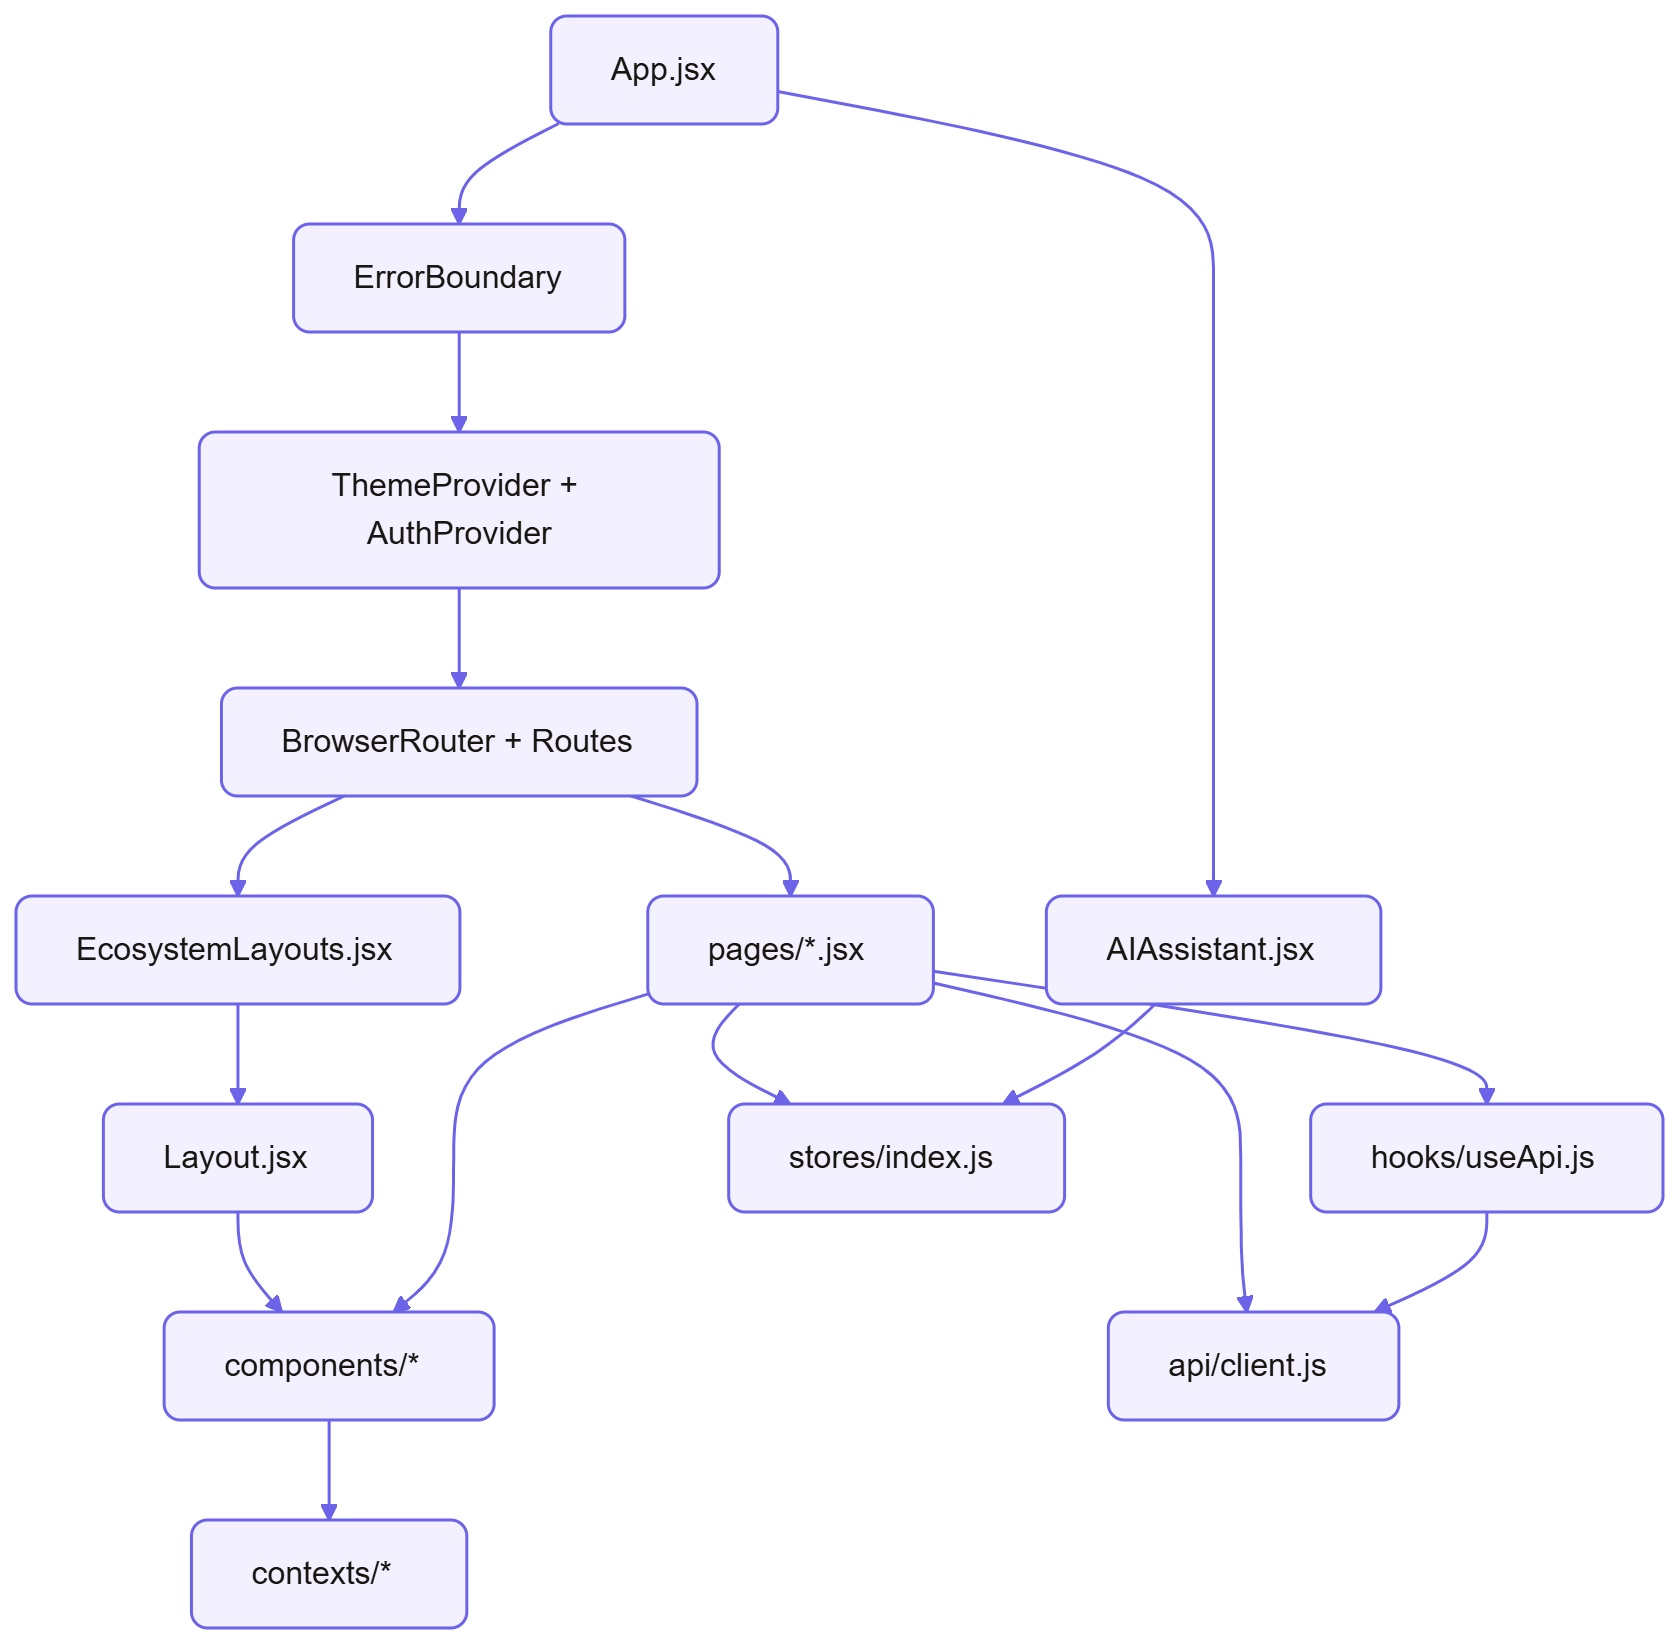
\includegraphics[width=0.7\textwidth]{Media/Chapter 4/2 React Component Architecture.jpg}
\caption{React Component Architecture of PrepSmart}
\label{fig:react_architecture}
\end{figure}

The React application is organized around a hierarchical component structure that separates application initialization, routing, layout management, reusable components, and API communication into independent modules.

The application execution begins from the App component, which acts as the entry point of the frontend application. The App component initializes the global providers, configures routing, and renders the major modules of the application.

Global state management is handled through the ThemeProvider and AuthProvider components. ThemeProvider maintains the application's appearance settings, including light and dark themes, while AuthProvider manages authentication state, user information, access tokens, and session persistence throughout the application.

Navigation within the application is implemented using BrowserRouter. Instead of loading separate HTML pages, BrowserRouter dynamically renders React components according to the current URL, thereby providing a seamless Single Page Application experience.

The Layout component provides a consistent user interface across different pages by managing the navigation bar, sidebar, footer, and common interface elements. Individual pages such as Dashboard, Learning Modules, Coding Practice, Interview Preparation, Company Readiness, Portfolio Management, and Profile Management are rendered within this layout.

Reusable UI components are organized separately from page-level components. These reusable components include cards, buttons, forms, charts, dialogs, tables, progress indicators, and visualization widgets that are shared across multiple pages, reducing code duplication and improving consistency.

Communication with the backend is centralized through the API Client module. Instead of making HTTP requests directly from individual pages, all API interactions are performed through a common client that automatically attaches authentication tokens, processes server responses, and handles error conditions consistently.

Application-wide state management is further supported through React Contexts and Stores. These modules maintain shared application data such as authentication status, dashboard information, user preferences, and placement preparation progress without requiring excessive component-to-component communication.

The frontend also integrates an AI Assistant component that provides intelligent assistance and interacts with backend AI services whenever supported functionality is available.

\subsection{Advantages of the Frontend Architecture}

The frontend architecture adopted in PrepSmart offers several advantages.

\begin{itemize}

\item Component-based development improves code reusability.

\item Single Page Application architecture provides faster navigation.

\item Centralized API communication simplifies backend integration.

\item Context Providers enable efficient global state management.

\item Reusable UI components improve maintainability.

\item Modular organization facilitates future feature expansion.

\item Dynamic rendering enhances user experience without full page reloads.

\end{itemize}

\section{Backend Implementation}

The backend of PrepSmart has been developed using Django and Django REST Framework (DRF), following a modular architecture that separates authentication, business logic, database operations, and API communication into independent components. The backend serves as the central processing unit of the platform by handling client requests, validating user permissions, executing application logic, interacting with the database, and generating structured JSON responses.

RESTful APIs are used as the communication mechanism between the React frontend and the Django backend. Each client request passes through authentication and validation before the corresponding business logic is executed. This architecture improves security, maintainability, and scalability while supporting efficient interaction between the frontend and backend.

Figure~\ref{fig:api_request_flow} illustrates the request processing workflow adopted in PrepSmart.

\begin{figure}[H]
\centering
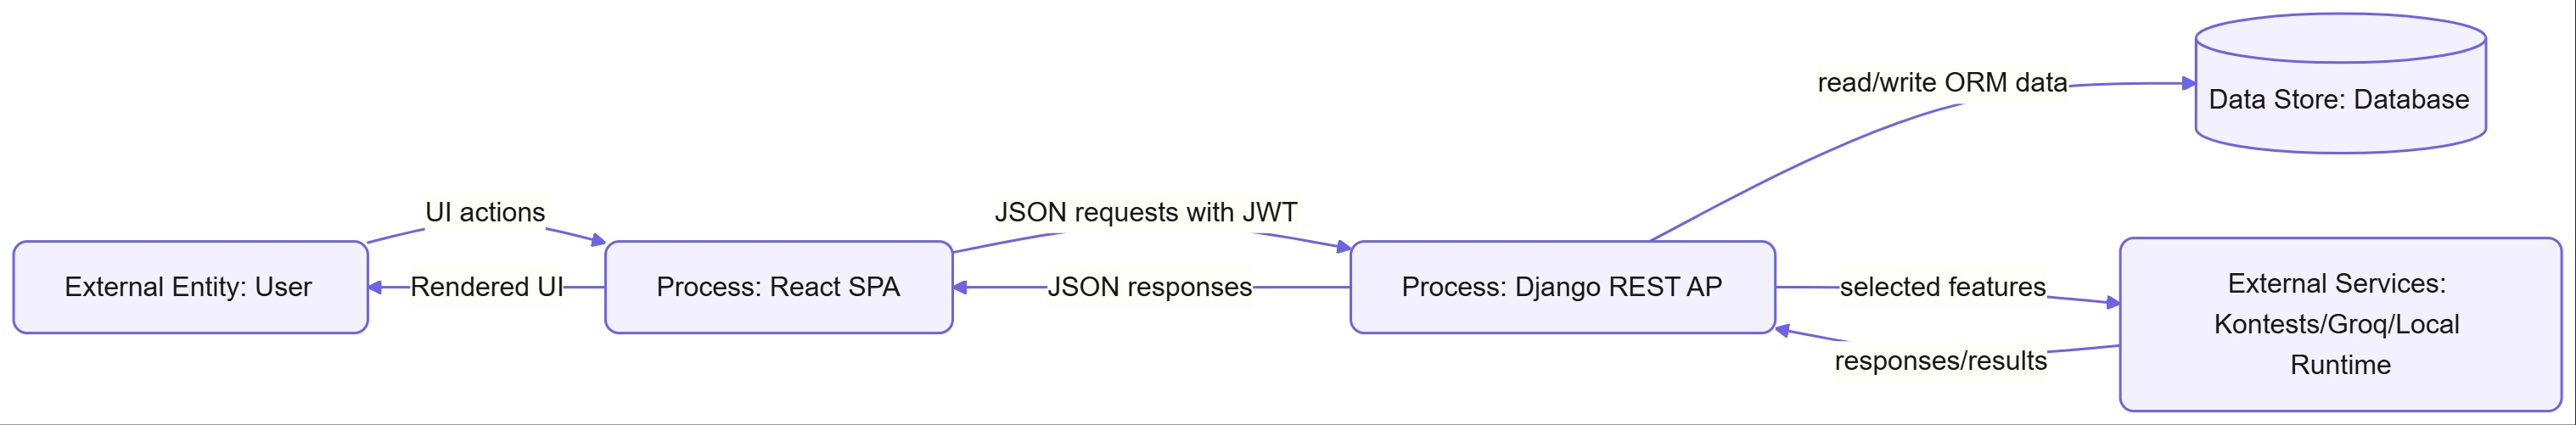
\includegraphics[width=\textwidth]{Media/Chapter 4/7 API Request Flow.jpg}
\caption{API Request Flow in PrepSmart}
\label{fig:api_request_flow}
\end{figure}

The API request processing begins when a user performs an action through the React frontend, such as logging into the system, starting a mock test, submitting code, or viewing dashboard statistics. The frontend sends an HTTP request through the centralized API Client using the appropriate REST endpoint.

The API Client automatically attaches the required HTTP headers, including the JSON Web Token (JWT) for authenticated requests. This ensures that protected resources are accessible only to authorized users.

The request is received by Django REST Framework, where authentication and permission checks are performed before forwarding the request to the appropriate API View. Each API View is responsible for processing a specific functionality of the platform, such as user authentication, topic management, coding practice, interview sessions, or dashboard analytics.

The API View interacts with Django ORM to retrieve or update application data stored in the relational database. Business rules, validation logic, and data processing are executed within the backend before generating the response.

Once processing is complete, the backend returns a structured JSON response containing the requested information or the execution result. The React frontend receives this response and dynamically updates the user interface without requiring a complete page refresh, thereby providing a responsive and seamless user experience.

\subsection{API Request Processing Workflow}

The request handling mechanism followed by PrepSmart consists of the following sequential steps:

\begin{enumerate}

\item The user performs an operation through the React web interface.

\item The API Client generates an HTTP request and attaches the necessary authentication headers.

\item Django REST Framework authenticates the request using JSON Web Tokens (JWT).

\item The request is forwarded to the corresponding API View.

\item The API View executes the required business logic.

\item Django ORM performs the required database operations.

\item The processed result is converted into a JSON response.

\item The frontend receives the response and updates the user interface dynamically.

\end{enumerate}

\subsection{Advantages of the Backend Architecture}

The backend implementation adopted in PrepSmart provides several advantages.

\begin{itemize}

\item Modular organization of backend services.

\item Secure RESTful communication using JWT authentication.

\item Efficient database interaction through Django ORM.

\item Separation of business logic from presentation logic.

\item Standardized JSON-based API communication.

\item Improved scalability through independent backend modules.

\item Easy integration with external APIs and AI services.

\end{itemize}

\section{Authentication Module}

Authentication is a fundamental component of the PrepSmart platform, ensuring that only authorized users can access protected resources and personalized placement preparation features. The system implements token-based authentication using JSON Web Tokens (JWT), providing a secure and scalable mechanism for user verification and session management.

The authentication module supports user registration, login, session validation, token refresh, and logout operations. Upon successful authentication, the backend generates an access token and a refresh token, which are securely managed by the frontend to maintain user sessions.

Figure~\ref{fig:authentication_sequence} illustrates the authentication workflow implemented in PrepSmart.

\begin{figure}[H]
\centering
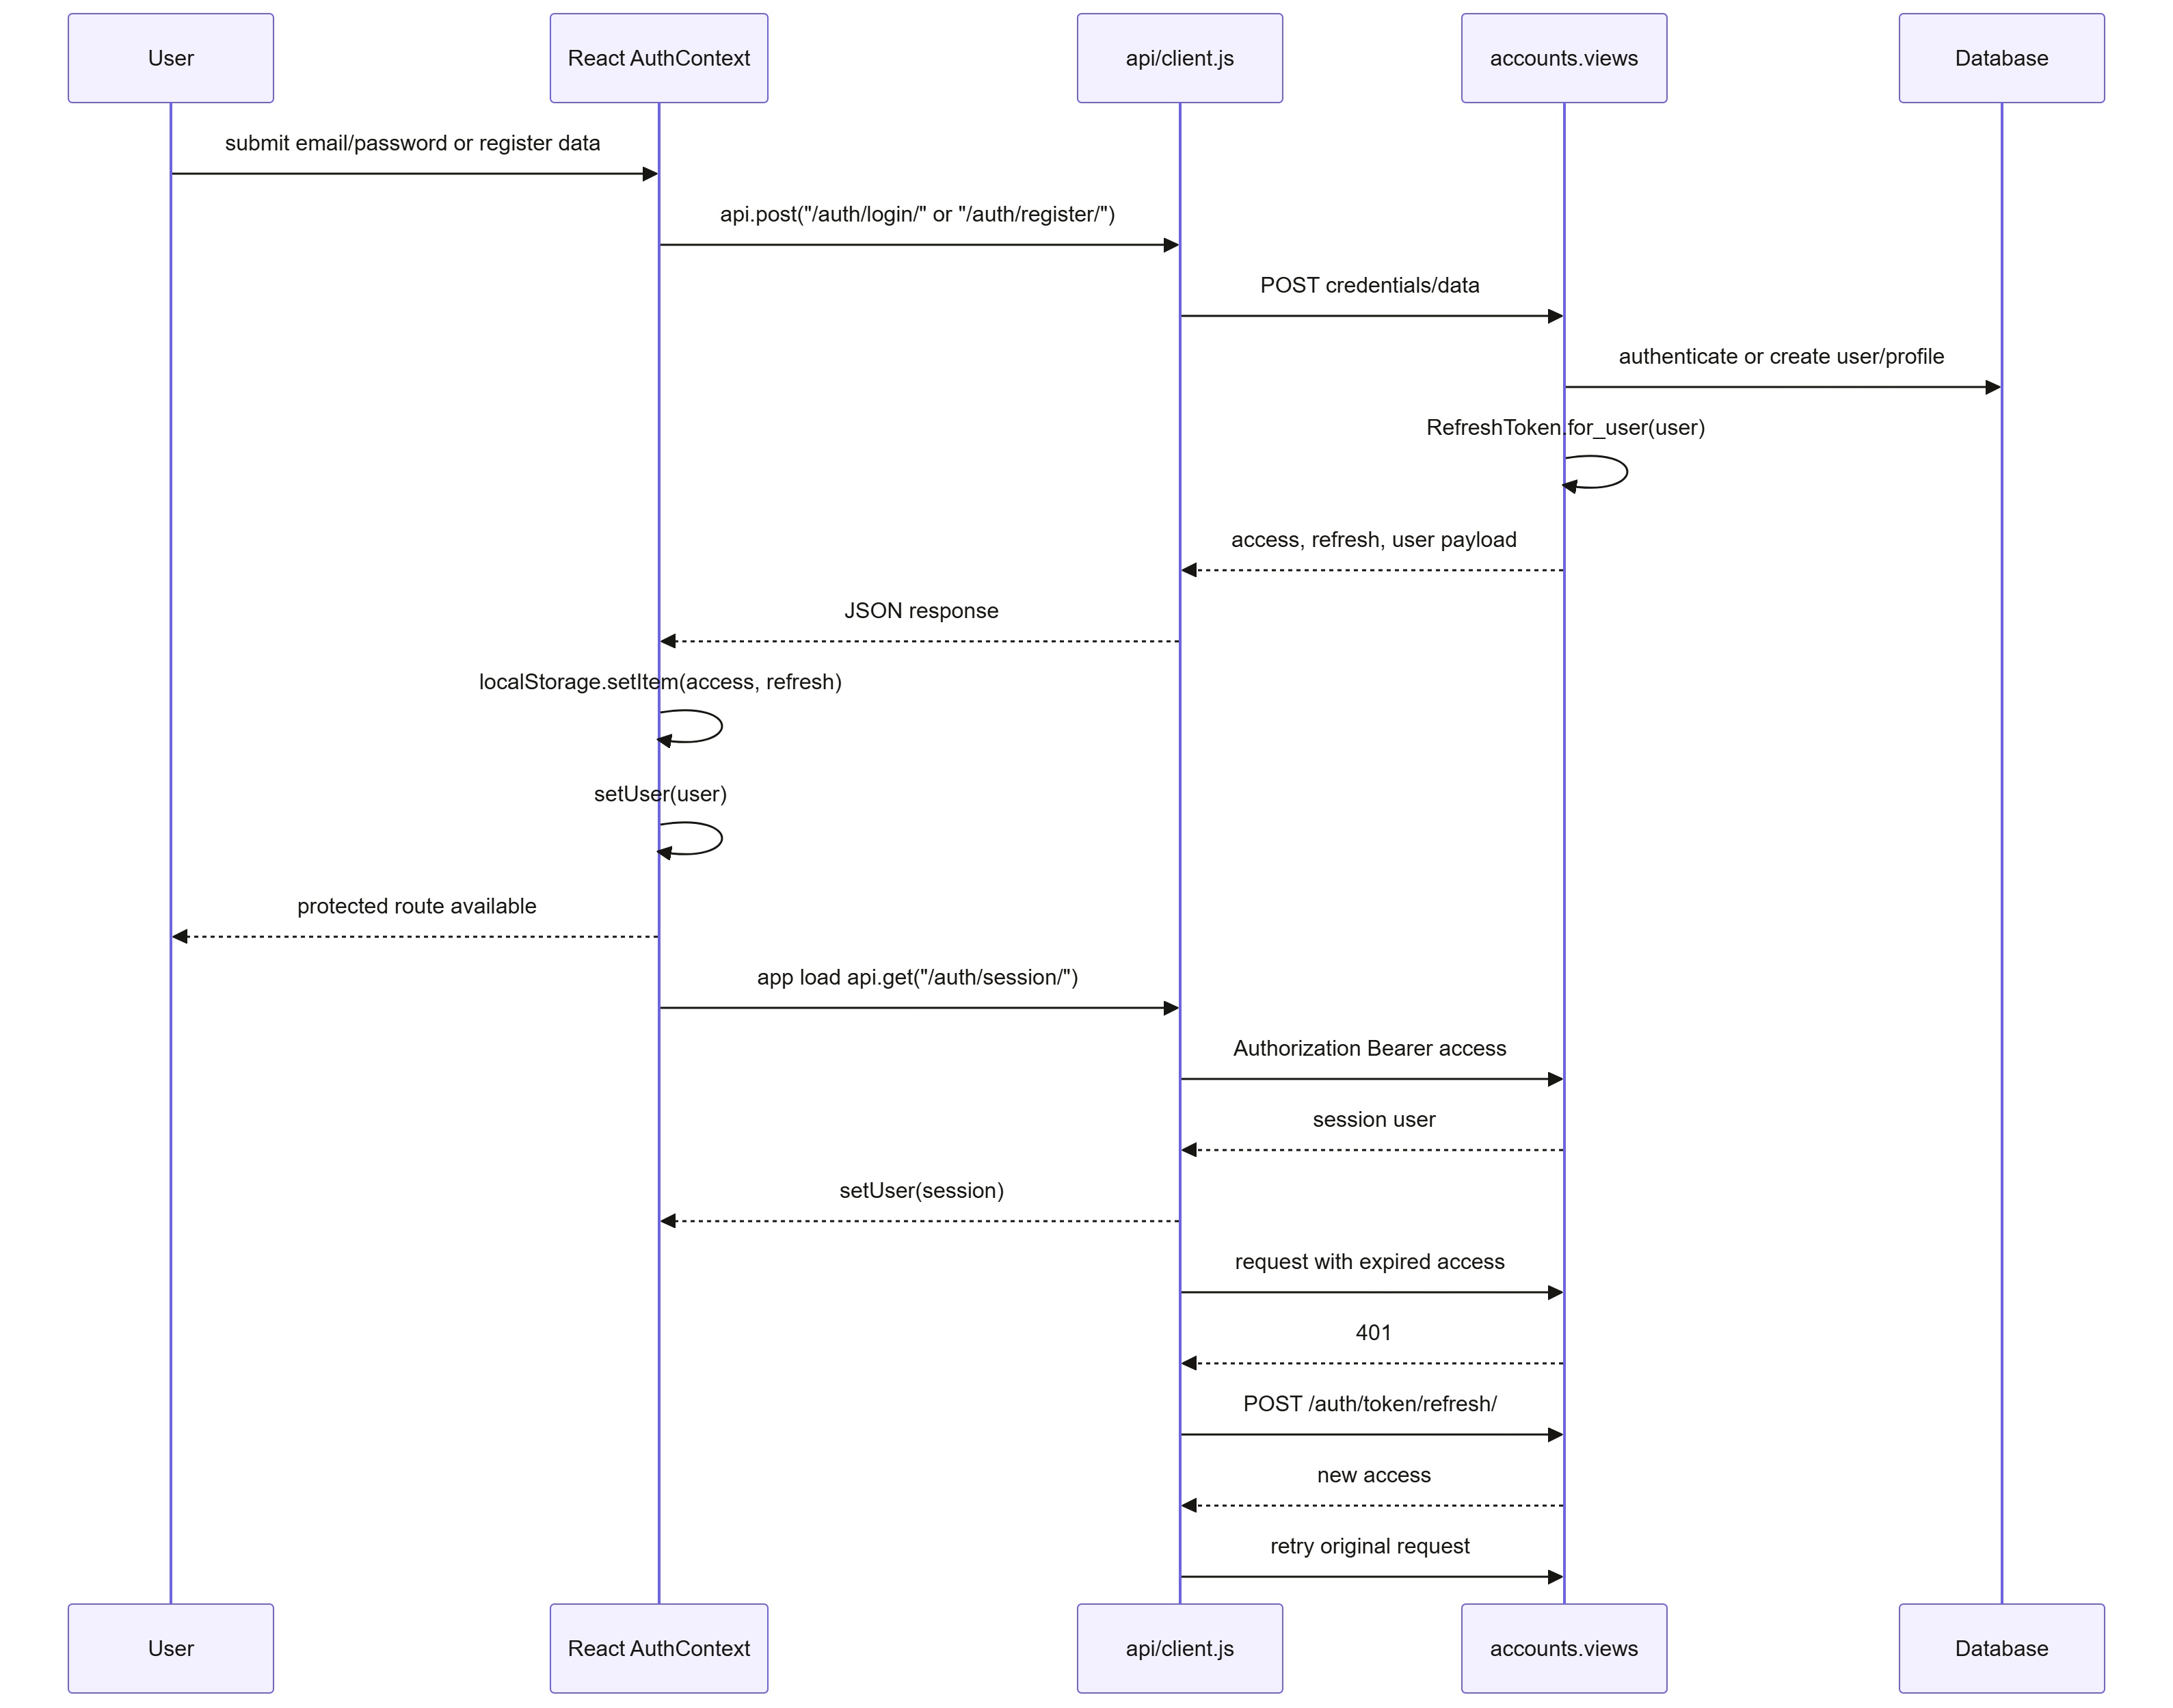
\includegraphics[width=0.83\textwidth]{Media/Chapter 4/9 Authentication Sequence.jpg}
\caption{Authentication Sequence Diagram of PrepSmart}
\label{fig:authentication_sequence}
\end{figure}

The authentication process begins when a user submits valid login credentials through the React frontend. The Auth Context forwards the credentials to the centralized API Client, which sends an authenticated HTTP POST request to the login endpoint exposed by Django REST Framework.

The backend verifies the supplied credentials against the stored user information in the database. If the credentials are valid, Django generates a JSON Web Token (JWT) pair consisting of an access token and a refresh token. Along with these tokens, the authenticated user's profile information is returned to the frontend.

The React application stores the received tokens securely in the browser's local storage and updates the authentication context with the logged-in user's information. Once authentication is successful, the user is redirected to the protected areas of the platform such as the dashboard, learning modules, coding workspace, and interview preparation pages.

Whenever the application starts, the frontend checks whether a valid user session already exists by requesting the session endpoint. If the access token is still valid, the backend returns the authenticated user's information and restores the session without requiring the user to log in again.

If an access token expires during API communication, the backend responds with an unauthorized status code. The API Client automatically sends the stored refresh token to the token refresh endpoint, receives a new access token, updates local storage, and retries the original request. This automatic refresh mechanism provides a seamless user experience while maintaining secure authentication throughout the application.

\subsection{Authentication Workflow}

The authentication mechanism implemented in PrepSmart follows the sequence below.

\begin{enumerate}

\item The user enters login credentials.

\item The frontend sends the credentials to the authentication API.

\item Django verifies the credentials using the user database.

\item A JWT access token and refresh token are generated.

\item Both tokens are returned to the frontend.

\item The frontend stores the tokens securely in local storage.

\item Protected API requests include the access token in the Authorization header.

\item If the access token expires, the refresh token is used to obtain a new access token.

\item The original API request is automatically retried without requiring the user to log in again.

\end{enumerate}

\subsection{Security Features}

The authentication module incorporates several security mechanisms to protect user accounts and application resources.

\begin{itemize}

\item Token-based authentication using JSON Web Tokens (JWT).

\item Secure separation of access tokens and refresh tokens.

\item Authentication of every protected API endpoint.

\item Automatic token refresh without interrupting the user session.

\item Prevention of unauthorized access through backend permission checks.

\item Session restoration after successful token validation.

\item Centralized authentication management using React Context.

\end{itemize}

\subsection{Advantages of the Authentication Module}

The implemented authentication mechanism provides several advantages.

\begin{itemize}

\item Secure user authentication.

\item Stateless communication between frontend and backend.

\item Reduced server-side session management.

\item Improved scalability for multiple concurrent users.

\item Seamless user experience through automatic token refresh.

\item Simplified integration with RESTful APIs.

\end{itemize}

\section{Placement Preparation Module}

The Placement Preparation Module forms the core functionality of the PrepSmart platform. It provides students with a structured learning journey that organizes placement preparation into tracks, topics, quizzes, coding exercises, and progress monitoring. The objective of this module is to guide students through a systematic learning process instead of relying on fragmented preparation across multiple platforms.

The module continuously records user activities, evaluates learning progress, and updates completion status after every learning activity. This enables students to monitor their preparation while allowing the system to generate personalized recommendations and readiness analytics.

Figure~\ref{fig:prep_journey} illustrates the workflow of the Placement Preparation Module.

\begin{figure}[H]
\centering
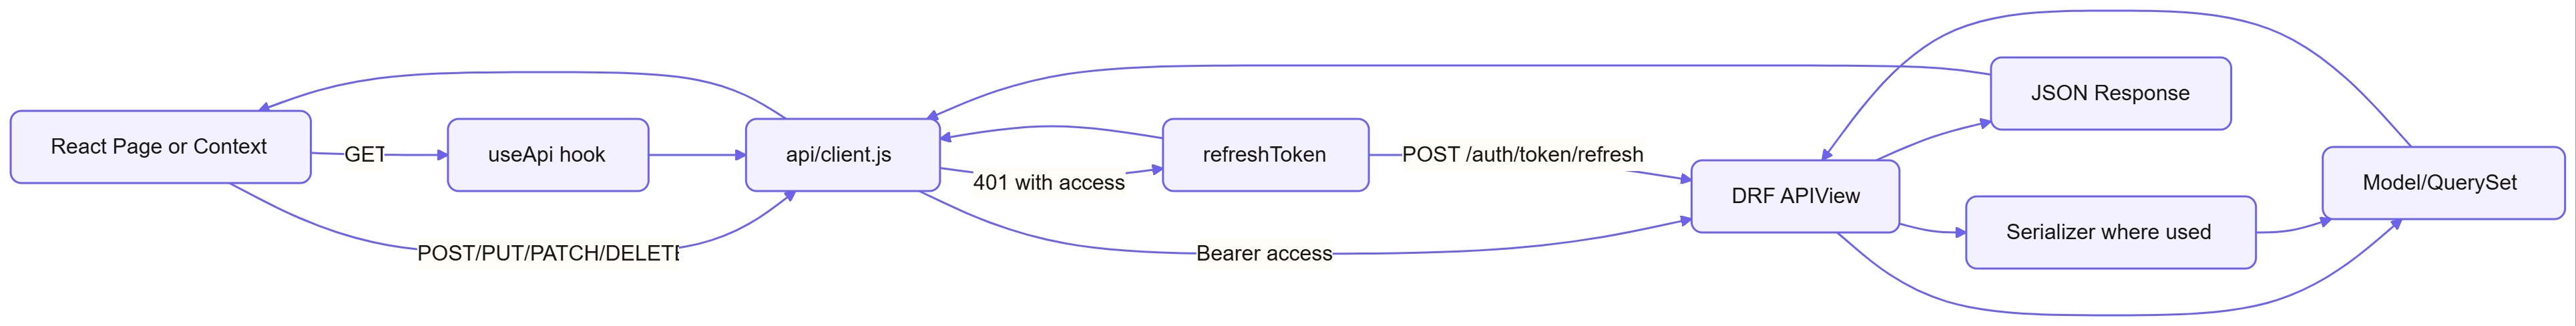
\includegraphics[width=\textwidth]{Media/Chapter 4/11 Preparation Journey Workflow.jpg}
\caption{Placement Preparation Workflow}
\label{fig:prep_journey}
\end{figure}

The placement preparation process begins when an authenticated student selects a learning track or topic from the frontend interface. The request is forwarded to the backend through the centralized API client, where the corresponding API endpoints process the request and retrieve the required learning content.

When a student completes a topic, the frontend sends a completion request to the backend. The backend verifies the authenticated user, retrieves the selected topic, and updates the corresponding learning progress record in the database. If the topic is being completed for the first time, the system creates a new progress entry and records the completion timestamp.

After completing the theoretical content, students attempt the topic quiz. Quiz responses are submitted to the backend, where each answer is evaluated against the stored correct answers. The backend calculates the student's accuracy and stores the result in the database. If the obtained score satisfies the predefined completion criteria, the corresponding topic is automatically marked as completed.

Every completed learning activity is recorded as an activity event, allowing the dashboard and analytics module to generate progress reports, calculate completion percentages, and recommend subsequent learning topics. This automated workflow ensures that students follow a structured placement preparation path while continuously tracking their overall readiness.

\subsection{Placement Preparation Workflow}

The Placement Preparation Module follows the workflow below.

\begin{enumerate}

\item The student selects a learning track.

\item The frontend requests the corresponding learning topics.

\item The backend retrieves topic information from the database.

\item The student studies the selected topic.

\item The student marks the topic as completed.

\item The backend updates the UserTopicProgress table.

\item The student attempts the topic quiz.

\item The backend evaluates quiz responses.

\item Progress statistics are updated.

\item Dashboard analytics are refreshed automatically.

\end{enumerate}

\subsection{Major Features}

The Placement Preparation Module provides the following features.

\begin{itemize}

\item Structured learning tracks.

\item Topic-wise study materials.

\item Quiz-based assessment.

\item Automatic progress tracking.

\item Activity logging.

\item Personalized learning journey.

\item Readiness score calculation.

\item Integration with dashboard analytics.

\end{itemize}

\subsection{Advantages of the Placement Preparation Module}

The implemented module offers several advantages.

\begin{itemize}

\item Organizes placement preparation into structured learning paths.

\item Eliminates fragmented learning across multiple platforms.

\item Automatically tracks student progress.

\item Provides continuous assessment through quizzes.

\item Enables personalized learning recommendations.

\item Supports future expansion with additional learning tracks.

\end{itemize}

\section{Dashboard and Analytics Module}

The Dashboard and Analytics Module provides students with a centralized view of their placement preparation progress. It aggregates learning activities, coding practice, quiz performance, interview readiness, company preparation, and daily goals into a single interactive dashboard. This enables students to monitor their overall progress and identify areas requiring improvement.

Figure~\ref{fig:dashboard_workflow} illustrates the workflow of the Dashboard and Analytics Module.

\begin{figure}[H]
\centering
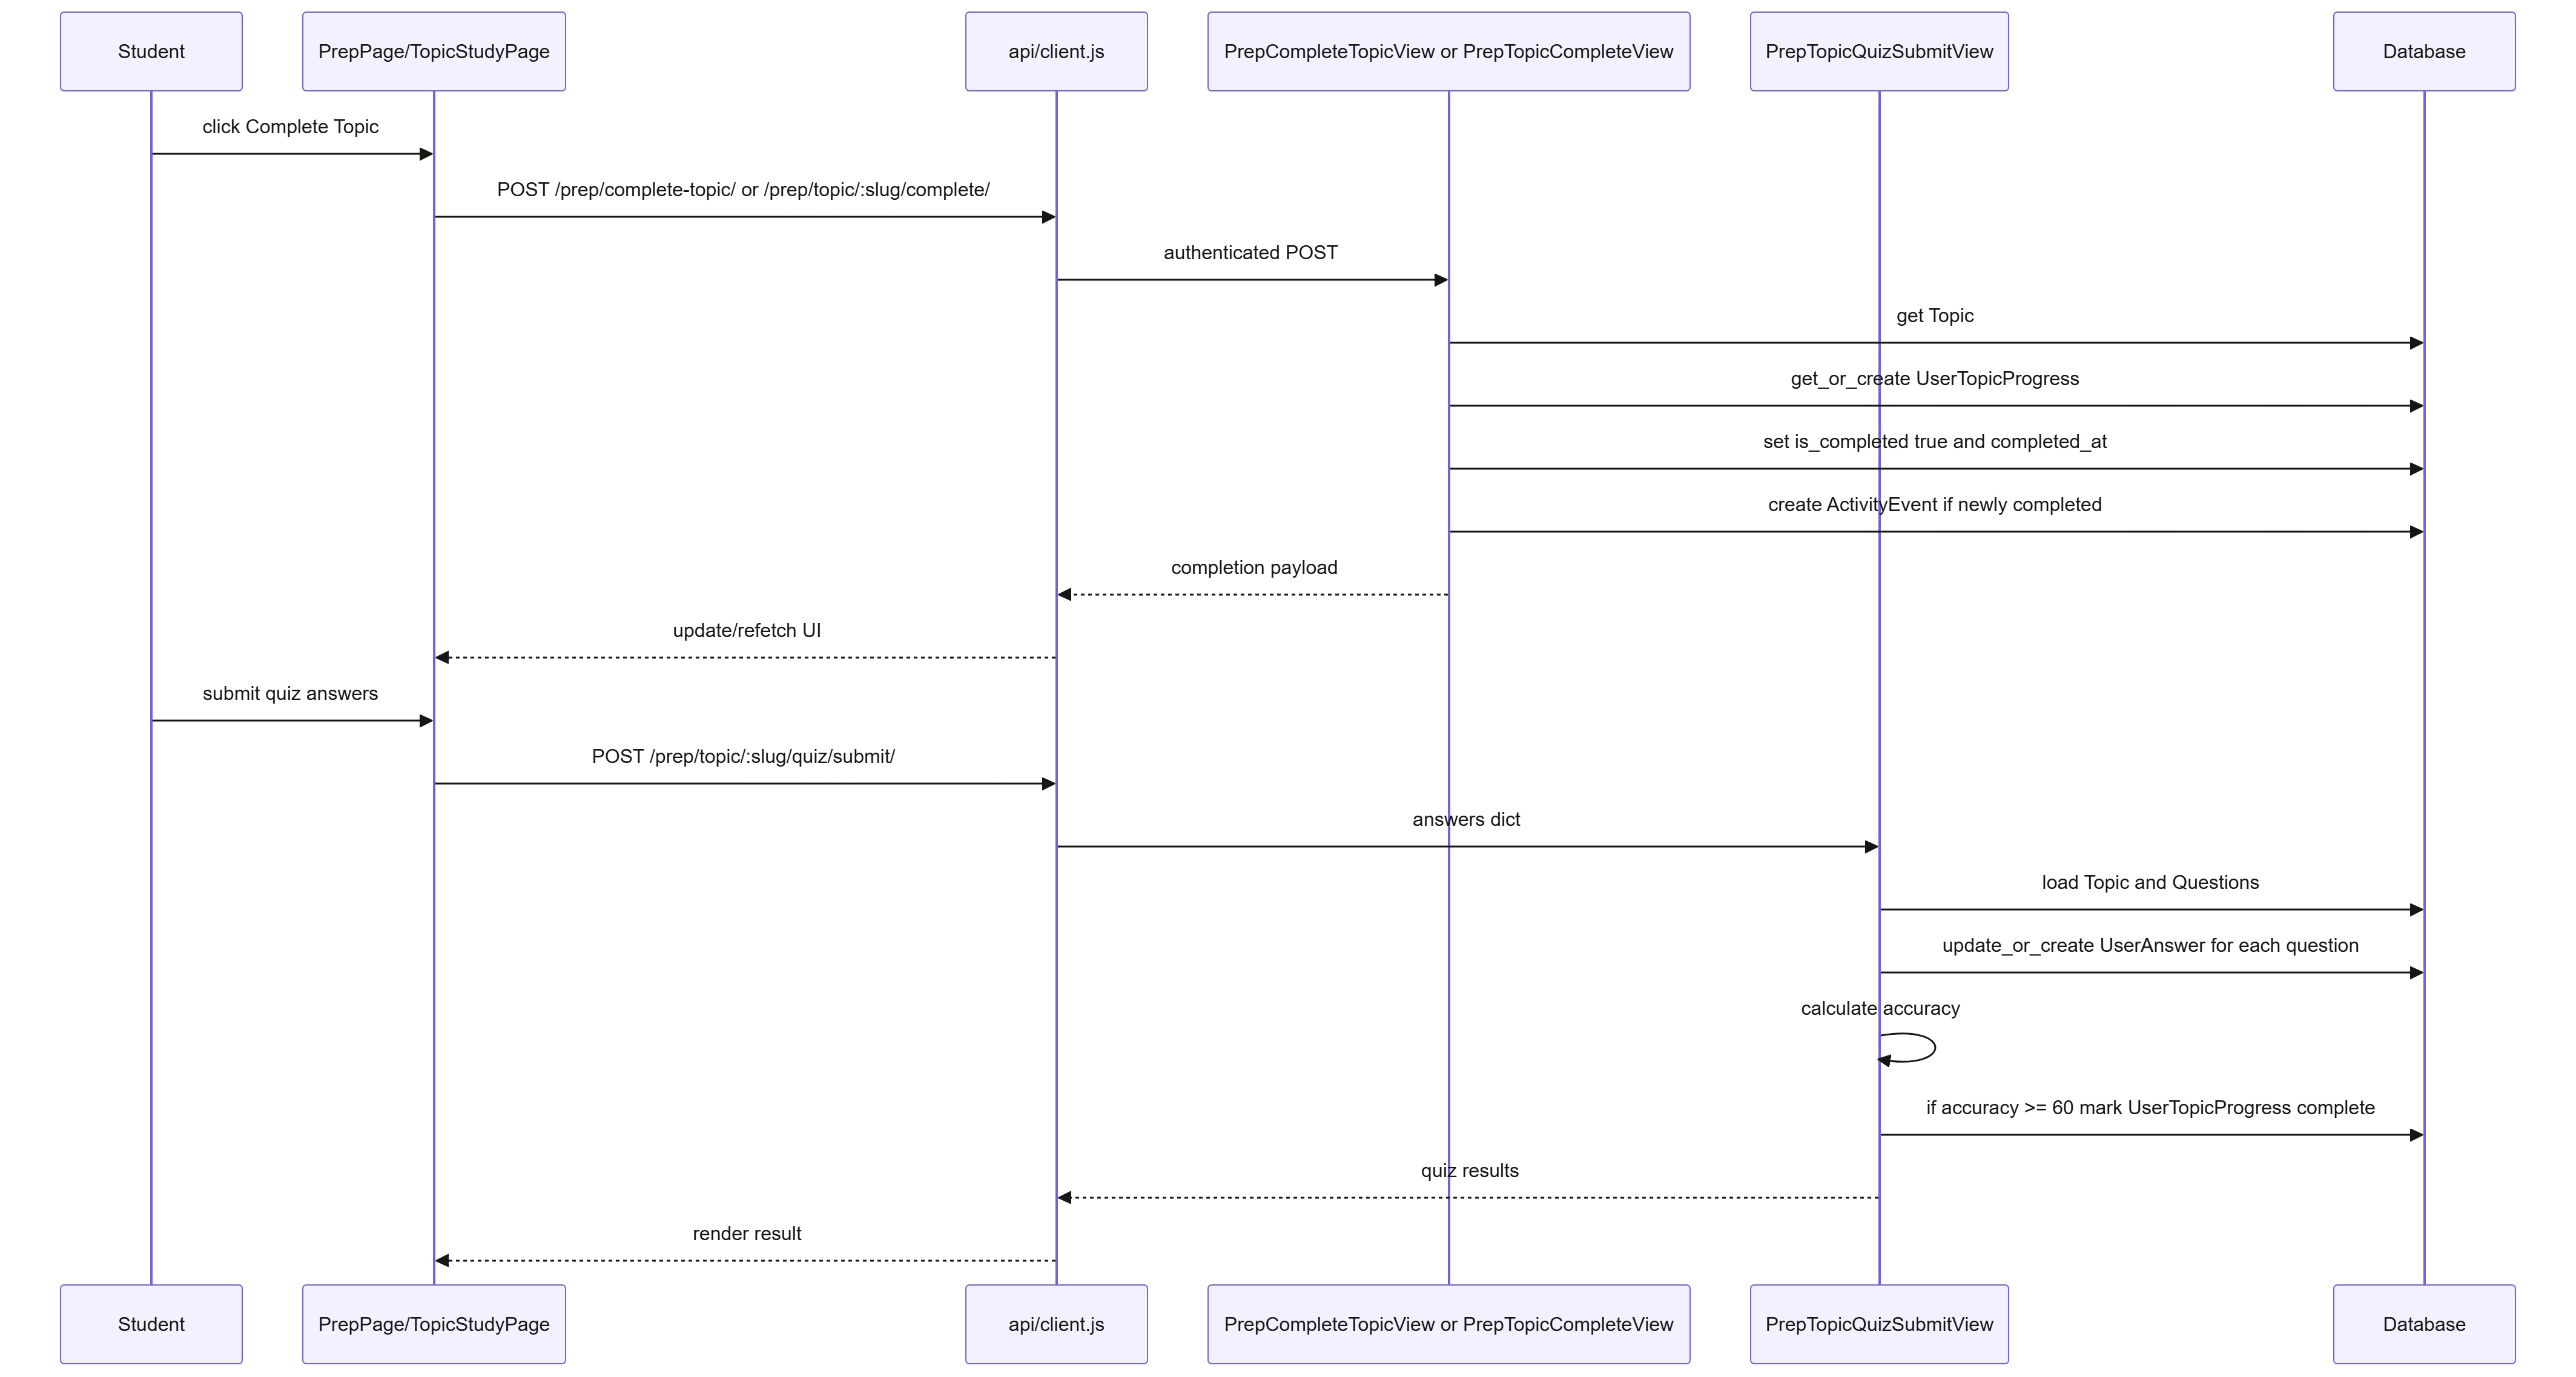
\includegraphics[width=\textwidth]{Media/Chapter 4/12 Dashboard Workflow.jpg}
\caption{Dashboard and Analytics Workflow}
\label{fig:dashboard_workflow}
\end{figure}

The dashboard is generated dynamically whenever an authenticated user accesses the application. The frontend requests dashboard information through the Dashboard API, which collects data from multiple backend modules.

The backend retrieves information related to user profiles, completed topics, quiz attempts, coding submissions, interview sessions, daily goals, revision schedules, company readiness records, and activity history. These records are processed to calculate important performance indicators such as completion percentage, quiz accuracy, coding statistics, interview readiness score, daily learning streak, and overall placement readiness.

The processed data is returned to the frontend as structured JSON responses. The React application visualizes this information using charts, progress indicators, summary cards, and statistical widgets. Since the dashboard retrieves live information from the database, users always receive updated analytics reflecting their latest activities.

The dashboard also serves as a personalized learning assistant by highlighting pending topics, revision requirements, upcoming milestones, and company-specific preparation status. This enables students to make informed decisions regarding their preparation strategy.

\subsection{Dashboard Features}

The Dashboard and Analytics Module provides the following features.

\begin{itemize}

\item Overall placement readiness score.

\item Topic-wise completion statistics.

\item Coding practice performance.

\item Quiz and mock test analysis.

\item Interview readiness tracking.

\item Company preparation progress.

\item Daily learning goals and streak monitoring.

\item Activity history and recent achievements.

\item Personalized learning recommendations.

\end{itemize}

\subsection{Advantages of the Dashboard Module}

The dashboard implementation offers several advantages.

\begin{itemize}

\item Centralized visualization of student progress.

\item Real-time performance analytics.

\item Continuous monitoring of placement readiness.

\item Easy identification of weak topics.

\item Motivation through progress tracking and learning streaks.

\item Integration of multiple learning modules into a unified analytical interface.

\end{itemize}

\section{Mock Test Module}

The Mock Test Module enables students to evaluate their preparation by attempting topic-wise assessments and milestone-based mock examinations. The module simulates actual placement examinations by providing timed tests, automatic evaluation, score calculation, and performance analysis.

The objective of this module is to help students identify weak areas, improve problem-solving speed, and continuously monitor their placement readiness through regular assessments.

Figure~\ref{fig:mock_test_workflow} illustrates the workflow of the Mock Test Module.

\begin{figure}[H]
\centering
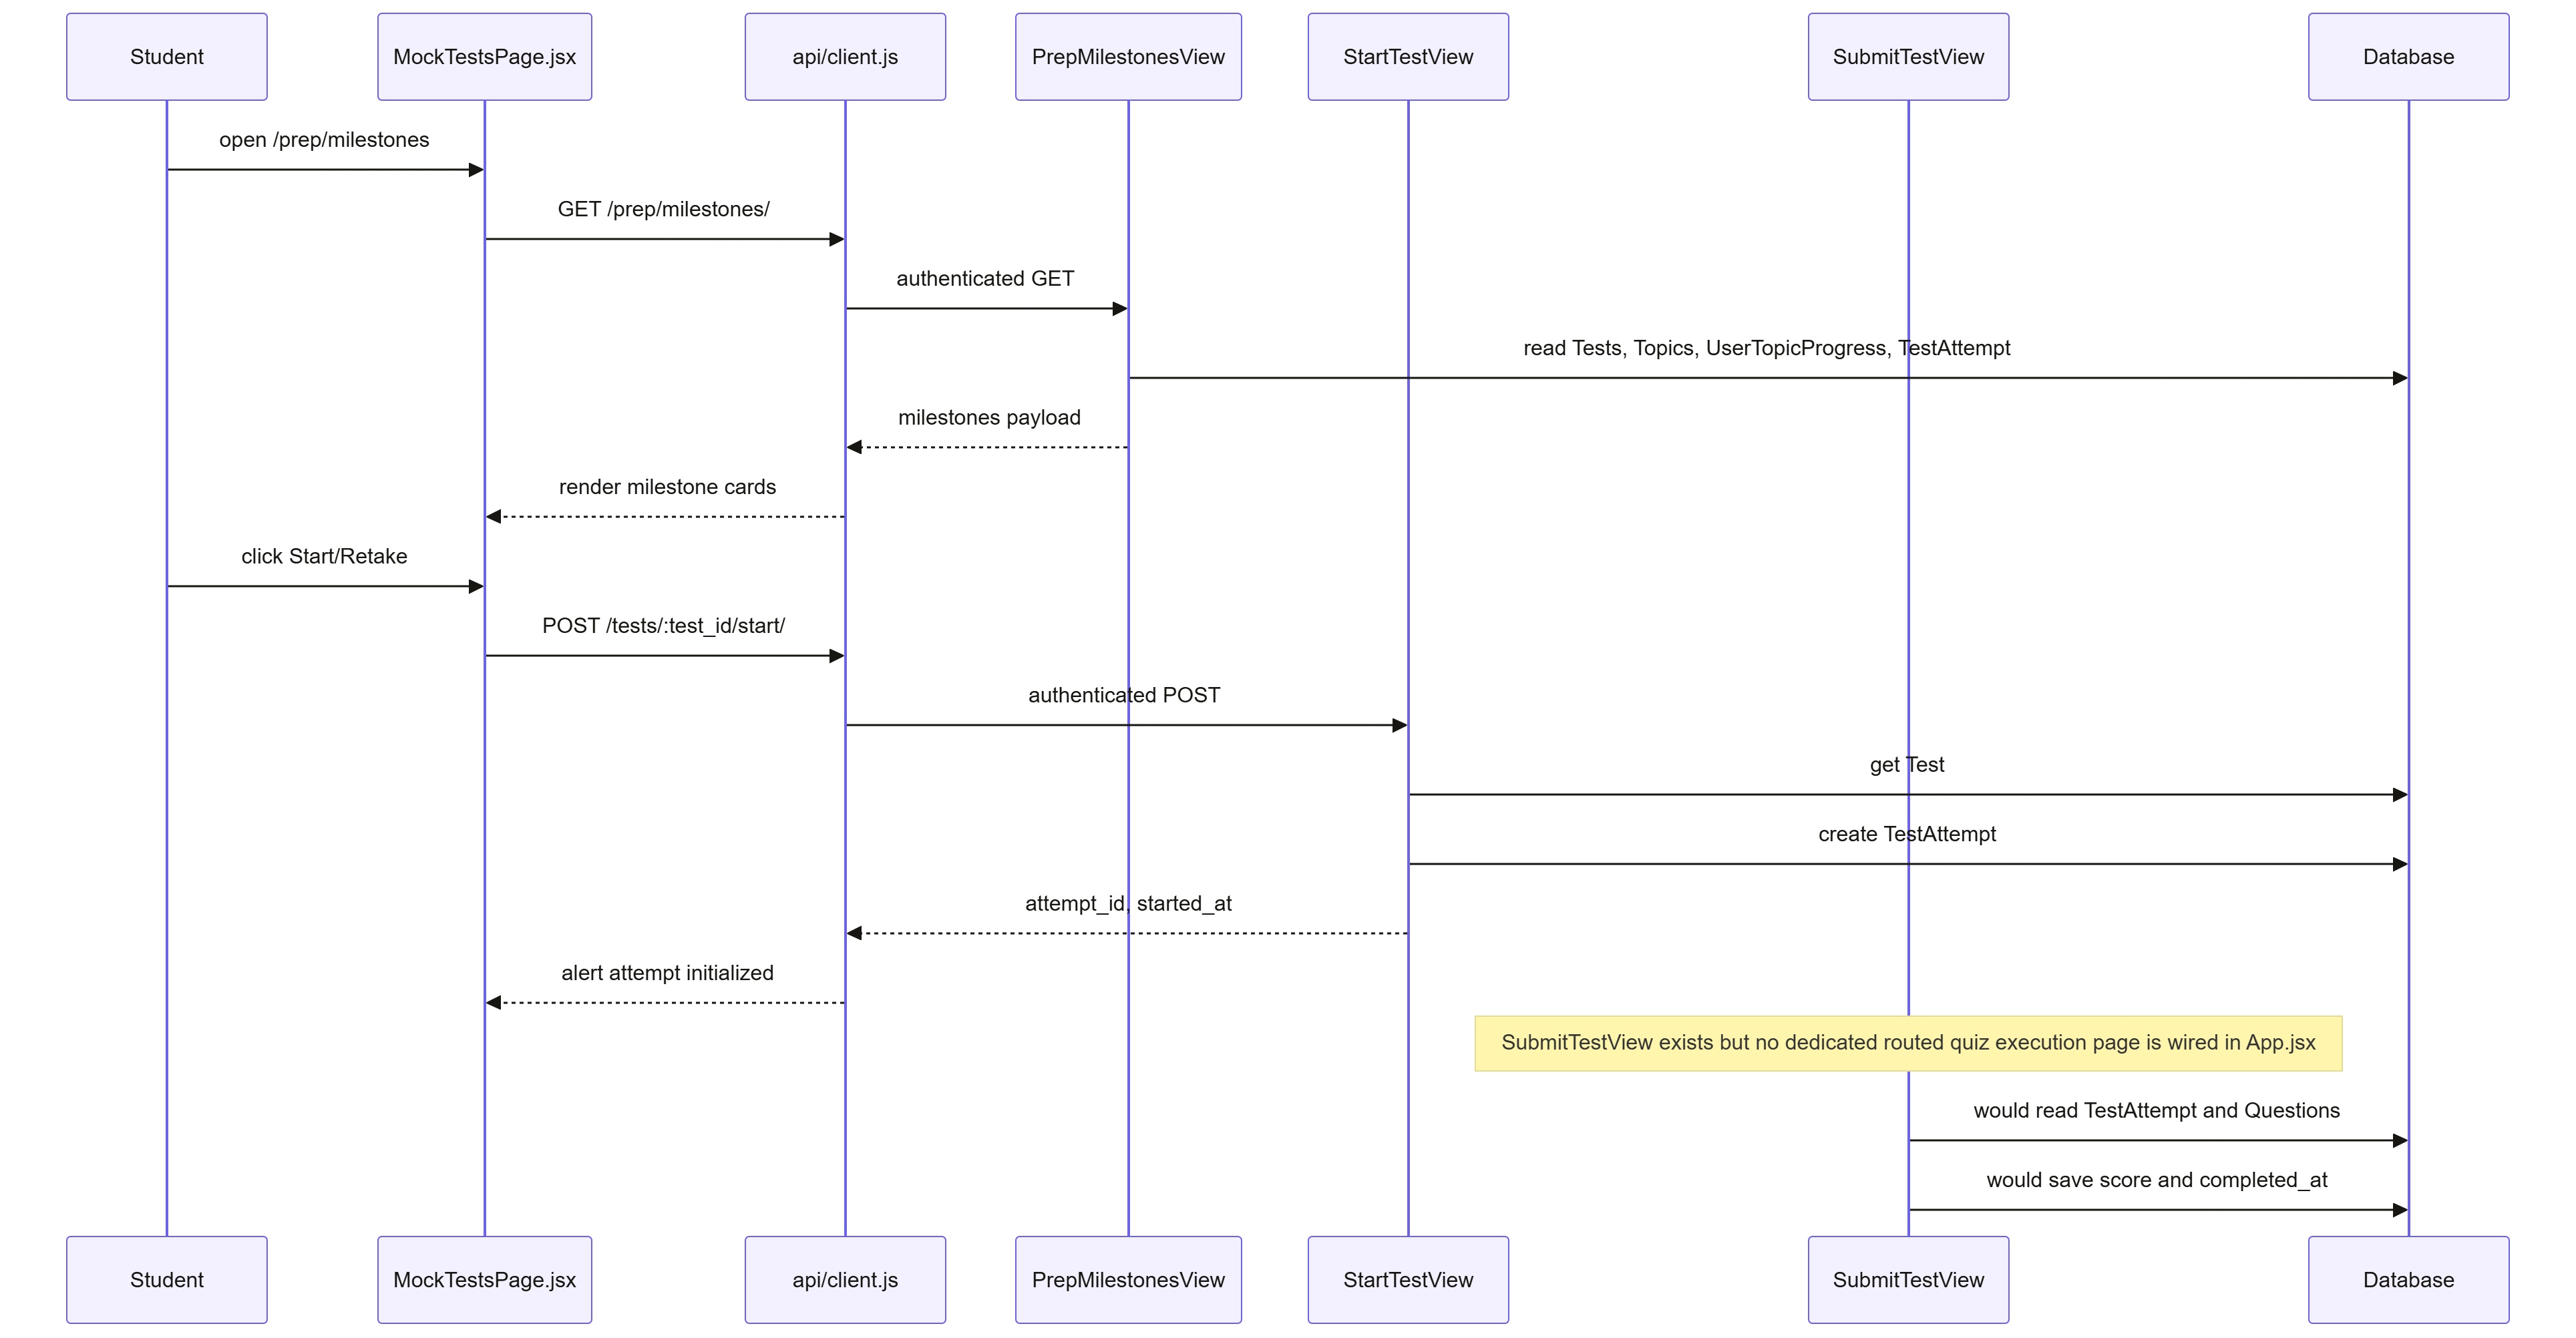
\includegraphics[width=\textwidth]{Media/Chapter 4/14 Mock Test Workflow.jpg}
\caption{Mock Test Workflow}
\label{fig:mock_test_workflow}
\end{figure}

The mock test process begins when an authenticated student selects a test from the available assessments displayed on the frontend. The React application requests the corresponding test details from the backend through the REST API.

The backend retrieves the selected test, associated topics, and question set from the database before creating a new TestAttempt record. This record stores the test identifier, start time, and user information, allowing the platform to track the student's progress throughout the assessment.

During the examination, students submit their answers through the frontend interface. The submitted responses are transmitted to the backend, where each answer is compared with the correct option stored in the database. The backend automatically calculates the obtained score, accuracy percentage, and other performance metrics before updating the TestAttempt record.

After evaluation, the calculated results are returned to the frontend and presented through scorecards, performance summaries, and topic-wise analysis. These results are also incorporated into the dashboard analytics module, enabling students to monitor their improvement over time and identify topics requiring additional practice.

\subsection{Mock Test Workflow}

The Mock Test Module follows the sequence below.

\begin{enumerate}

\item The student selects a mock test.

\item The frontend requests the test details.

\item The backend retrieves questions from the database.

\item A new TestAttempt record is created.

\item The student submits answers.

\item The backend evaluates each response.

\item The final score and statistics are calculated.

\item Results are stored in the database.

\item Performance analytics are updated.

\item The frontend displays the scorecard and analysis.

\end{enumerate}

\subsection{Major Features}

The Mock Test Module provides the following features.

\begin{itemize}

\item Topic-wise assessments.

\item Timed examinations.

\item Automatic evaluation.

\item Instant score generation.

\item Accuracy calculation.

\item Performance history.

\item Dashboard integration.

\item Continuous placement readiness assessment.

\end{itemize}

\subsection{Advantages of the Mock Test Module}

The implemented module provides several benefits.

\begin{itemize}

\item Simulates real placement examinations.

\item Provides immediate performance feedback.

\item Identifies weak learning areas.

\item Improves examination confidence.

\item Enables continuous progress tracking.

\item Supports data-driven preparation strategies.

\end{itemize}

\section{AI Interview Module}

The AI Interview Module is designed to simulate technical interview sessions and help students improve their communication, problem-solving, and technical knowledge. Unlike traditional question banks, this module provides an interactive interview experience by presenting questions, collecting responses, evaluating answers, and generating intelligent feedback using Artificial Intelligence.

The module supports different interview categories and maintains complete interview history, enabling students to monitor their progress over multiple interview sessions.

Figure~\ref{fig:ai_interview_workflow} illustrates the workflow of the AI Interview Module.

\begin{figure}[H]
\centering
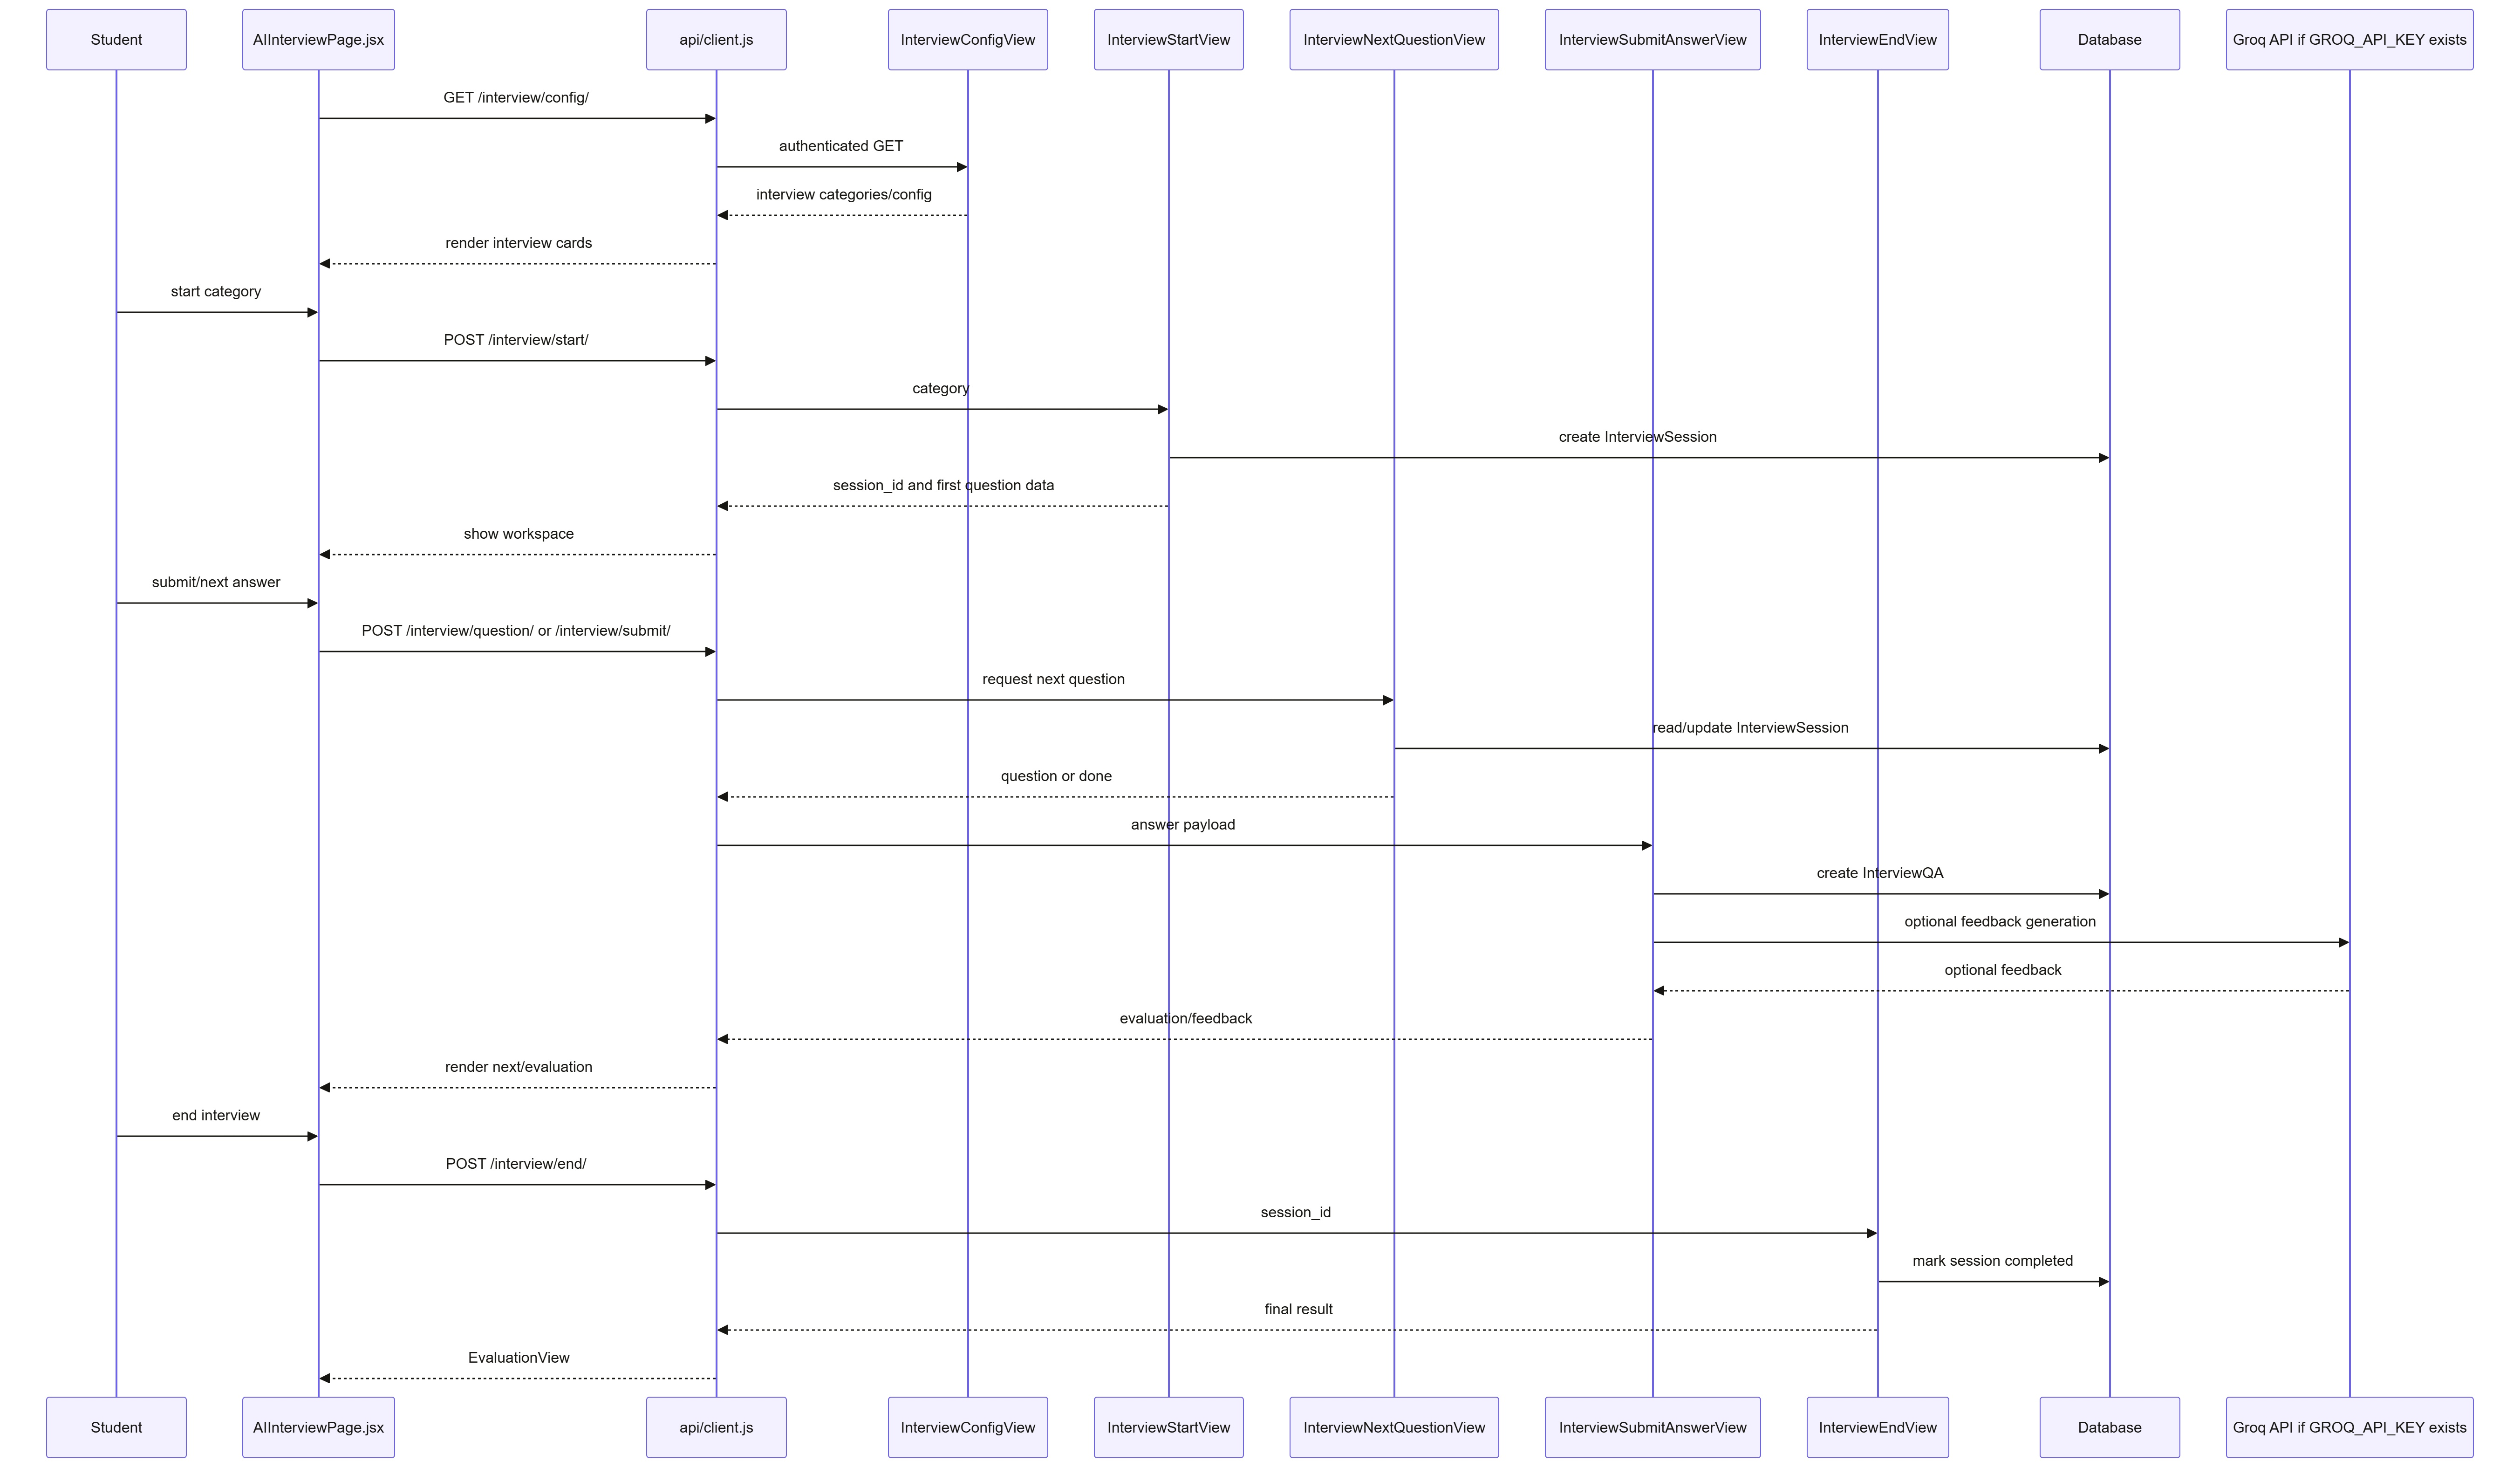
\includegraphics[width=\textwidth]{Media/Chapter 4/15 AI Interview Workflow.jpg}
\caption{AI Interview Workflow}
\label{fig:ai_interview_workflow}
\end{figure}

The AI Interview Module begins when an authenticated student selects an interview category through the frontend interface. The React application requests the available interview configuration from the backend, including interview categories and question settings.

After the interview configuration is loaded, the student starts a new interview session. The backend creates an InterviewSession record in the database and returns the first interview question to the frontend. Throughout the interview, each submitted response is transmitted to the backend for processing and evaluation.

The backend records every question and corresponding user response in the InterviewQA table. When AI functionality is enabled, the submitted answer is forwarded to the Groq API, which generates feedback regarding correctness, communication quality, technical depth, and possible improvements.

The generated feedback is returned to the frontend and displayed immediately after each response or at the end of the interview session, depending on the interview configuration. The backend also calculates interview scores and stores the final interview result, allowing students to review previous interview sessions and monitor their overall interview readiness.

\subsection{AI Interview Workflow}

The AI Interview Module follows the sequence below.

\begin{enumerate}

\item The student selects an interview category.

\item The frontend requests interview configuration.

\item The backend creates a new InterviewSession.

\item The first interview question is displayed.

\item The student submits an answer.

\item The backend records the response.

\item The answer is evaluated using backend logic and AI services.

\item Feedback and evaluation scores are generated.

\item The interview continues until all questions are completed.

\item The final interview report is stored and displayed.

\end{enumerate}

\subsection{Major Features}

The AI Interview Module provides the following features.

\begin{itemize}

\item Category-based interview sessions.

\item AI-assisted answer evaluation.

\item Automated interview scoring.

\item Detailed feedback generation.

\item Interview history management.

\item Readiness assessment.

\item Backend integration using REST APIs.

\item Secure storage of interview records.

\end{itemize}

\subsection{Advantages of the AI Interview Module}

The AI Interview Module offers several advantages.

\begin{itemize}

\item Simulates real technical interview experiences.

\item Provides immediate AI-generated feedback.

\item Improves communication and technical skills.

\item Enables continuous interview practice.

\item Tracks interview performance over time.

\item Supports personalized placement preparation.

\end{itemize}

\section{Coding Practice Module}

The Coding Practice Module enables students to solve programming problems directly within the PrepSmart platform. It provides an integrated coding environment where users can write, execute, and submit solutions without relying on external programming websites. The module supports multiple programming languages, automatic code evaluation, execution statistics, and result visualization.

The primary objective of this module is to strengthen problem-solving skills by providing an environment similar to technical coding interviews and online programming assessments.

Figure~\ref{fig:coding_workflow} illustrates the workflow of the Coding Practice Module.

\begin{figure}[H]
\centering
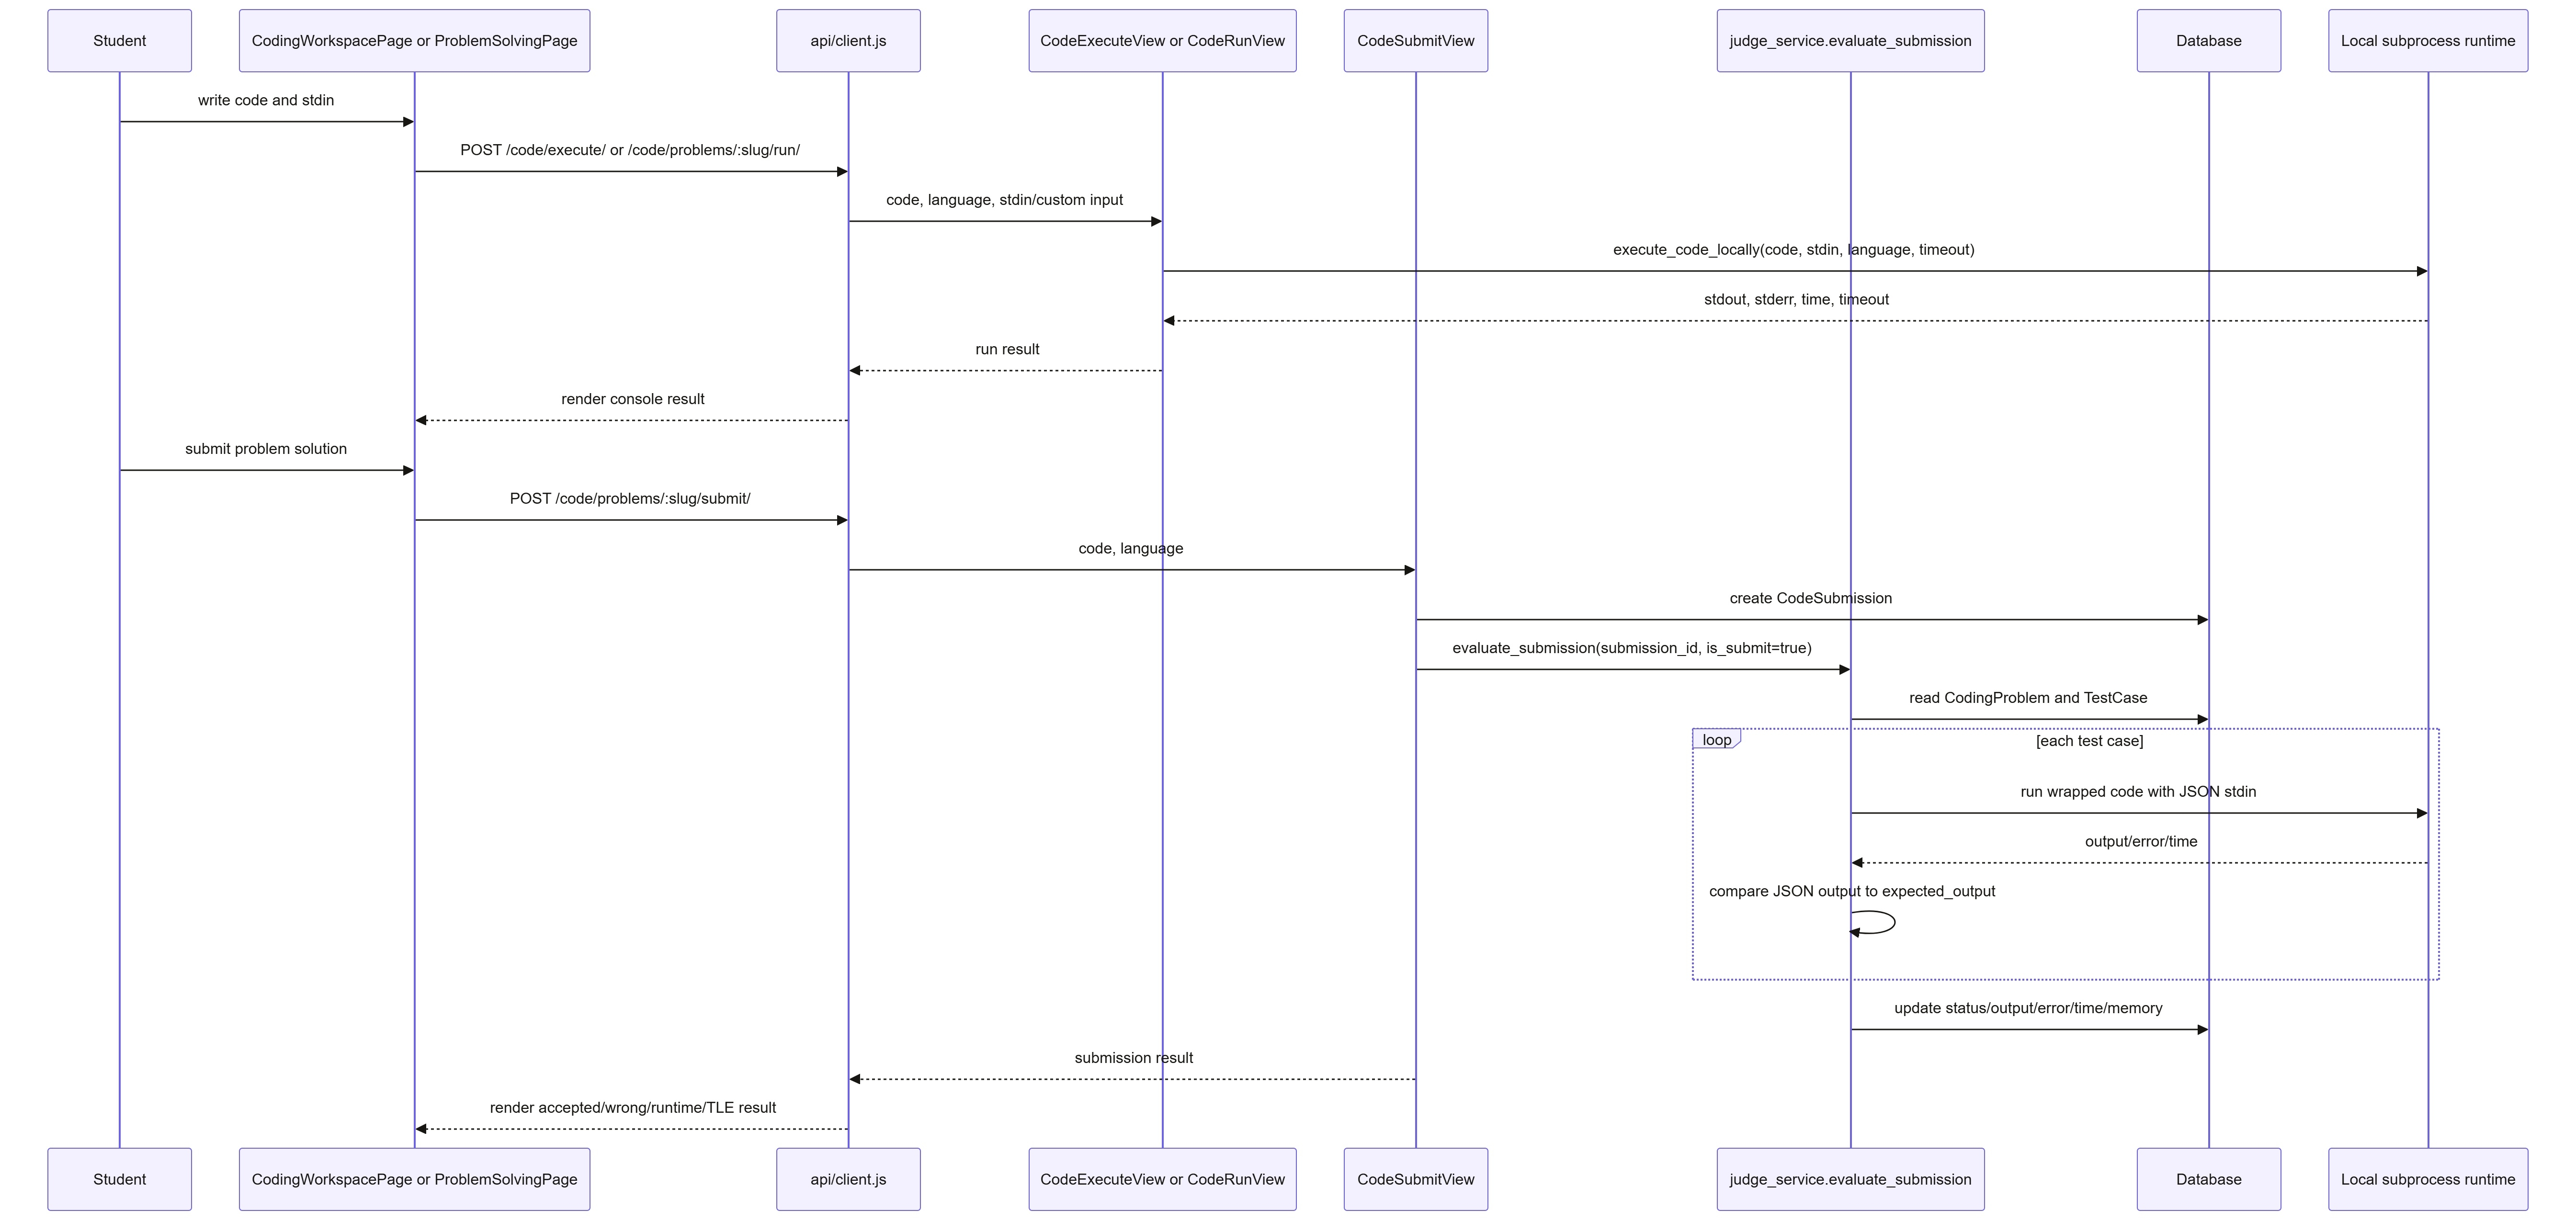
\includegraphics[width=\textwidth]{Media/Chapter 4/16 Coding Execution Workflow.jpg}
\caption{Coding Practice Workflow}
\label{fig:coding_workflow}
\end{figure}

The coding workflow begins when an authenticated student selects a programming problem from the coding workspace. The frontend retrieves the problem statement, constraints, supported programming languages, and starter code from the backend through REST APIs.

The student writes the solution using the integrated code editor and may execute the program using custom input before final submission. For execution requests, the frontend sends the source code, selected programming language, and input data to the backend.

The backend forwards the request to the local code execution engine, which compiles and executes the submitted program inside a controlled subprocess environment. During execution, the system records standard output, error messages, execution time, memory usage, and timeout status.

When the student submits the solution, a new CodeSubmission record is created in the database. The backend invokes the evaluation service, which executes the submitted program against all predefined test cases associated with the selected coding problem. The generated output is compared with the expected output for every test case to determine whether the solution is accepted.

After evaluation, the backend updates the submission status, execution statistics, runtime information, and evaluation result before returning the complete report to the frontend. The React application displays the evaluation outcome, enabling students to analyze errors, improve their solutions, and continue practicing programming problems.

\subsection{Coding Practice Workflow}

The Coding Practice Module follows the sequence below.

\begin{enumerate}

\item The student selects a programming problem.

\item The frontend retrieves the problem details.

\item The student writes source code using the integrated editor.

\item The code is executed using custom input when required.

\item The backend compiles and executes the program.

\item Execution statistics are collected.

\item The student submits the final solution.

\item The backend evaluates the solution against all test cases.

\item Submission results are stored in the database.

\item The frontend displays the final evaluation report.

\end{enumerate}

\subsection{Major Features}

The Coding Practice Module provides the following features.

\begin{itemize}

\item Integrated online code editor.

\item Support for multiple programming languages.

\item Custom input execution.

\item Automatic compilation and execution.

\item Test case based evaluation.

\item Runtime and memory analysis.

\item Submission history.

\item Secure local code execution environment.

\end{itemize}

\subsection{Advantages of the Coding Practice Module}

The Coding Practice Module provides several advantages.

\begin{itemize}

\item Provides an interview-like programming environment.

\item Enables immediate execution and evaluation of solutions.

\item Helps students improve coding efficiency.

\item Supports continuous programming practice.

\item Automatically records submission history.

\item Integrates coding performance with dashboard analytics.

\end{itemize}

\section{Portfolio and Skills Passport Module}

The Portfolio and Skills Passport Module enables students to build a professional digital profile that showcases their academic achievements, technical skills, projects, certifications, and overall placement readiness. Unlike traditional resumes, the module dynamically generates a structured portfolio and an employability passport using information already available within the PrepSmart platform.

The module also supports public sharing of portfolios through unique URLs, allowing recruiters and placement coordinators to review student profiles without requiring access to the internal system.

Figure~\ref{fig:portfolio_workflow} illustrates the workflow of the Portfolio and Skills Passport Module.

\begin{figure}[H]
\centering
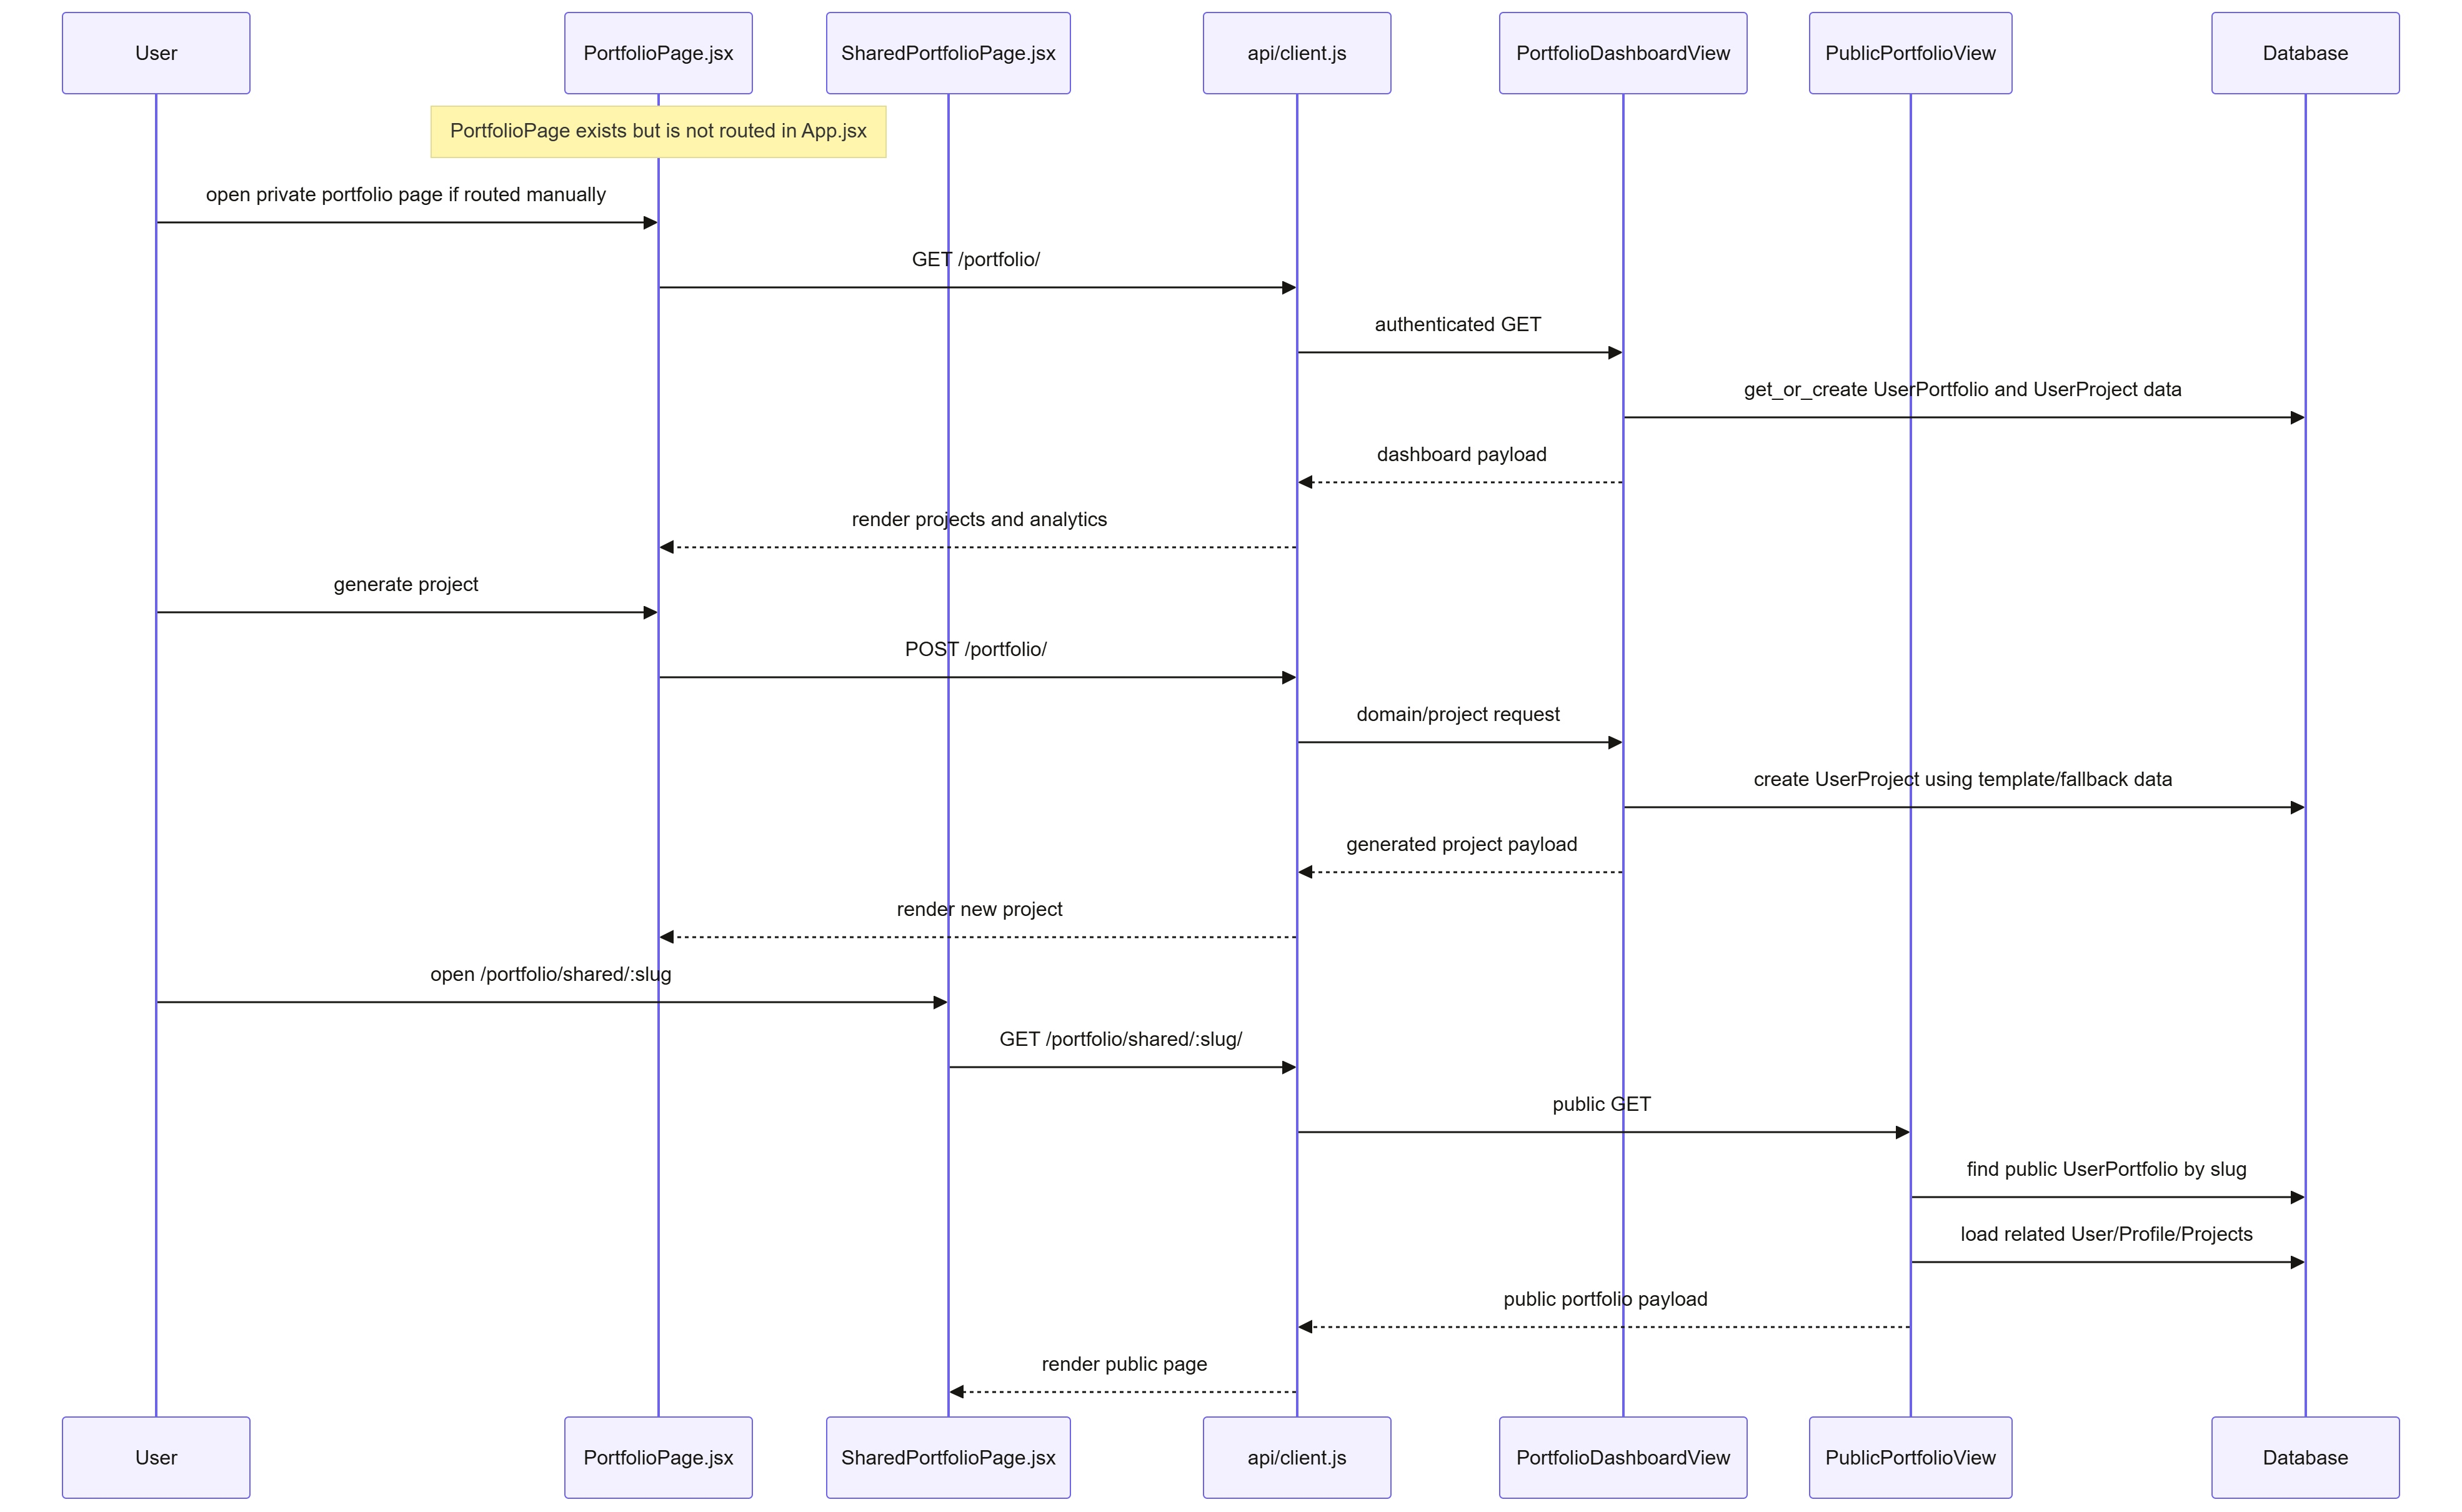
\includegraphics[width=\textwidth]{Media/Chapter 4/17 Portfolio Workflow.jpg}
\caption{Portfolio and Skills Passport Workflow}
\label{fig:portfolio_workflow}
\end{figure}

The Portfolio and Skills Passport Module begins when an authenticated student accesses the portfolio section through the frontend interface. The React application sends a request to the backend to retrieve the user's academic information, projects, certifications, technical skills, coding statistics, interview performance, and placement preparation progress.

The backend collects the required information from multiple database entities, including UserProfile, UserProject, UserCertificate, UserPassport, UserPortfolio, and other related records. These data are processed to generate a comprehensive professional profile representing the student's overall employability.

Students can further customize their portfolio by adding project descriptions, technology stacks, GitHub links, and personal achievements. The backend stores these modifications and generates a unique public URL that can be shared with recruiters or placement coordinators.

The Skills Passport is generated automatically using analytical information collected throughout the placement preparation journey. Metrics such as coding performance, interview readiness, learning progress, and technical competency are consolidated into a unified employability profile that reflects the student's current preparation status.

Whenever a recruiter or external user accesses a shared portfolio or passport link, the backend retrieves only publicly available information and renders the corresponding profile without exposing confidential user data.

\subsection{Portfolio Generation Workflow}

The Portfolio and Skills Passport Module follows the workflow below.

\begin{enumerate}

\item The student accesses the portfolio dashboard.

\item The frontend requests portfolio information.

\item The backend retrieves academic and placement data.

\item Portfolio information is generated dynamically.

\item Skills Passport metrics are calculated.

\item Public sharing links are generated.

\item Portfolio information is stored in the database.

\item Shared portfolios are displayed to authorized external users.

\end{enumerate}

\subsection{Major Features}

The Portfolio and Skills Passport Module provides the following features.

\begin{itemize}

\item Automatic portfolio generation.

\item Skills Passport generation.

\item Public portfolio sharing.

\item Project management.

\item Certification management.

\item Recruiter-friendly profile presentation.

\item Dynamic employability score generation.

\item Integration with placement analytics.

\end{itemize}

\subsection{Advantages of the Portfolio and Skills Passport Module}

The implemented module offers several advantages.

\begin{itemize}

\item Eliminates manual portfolio preparation.

\item Automatically reflects placement preparation progress.

\item Improves recruiter visibility.

\item Provides a centralized professional profile.

\item Supports public sharing through secure URLs.

\item Encourages continuous profile improvement.

\end{itemize}

\section{Company Readiness Module}

The Company Readiness Module assists students in preparing for specific companies by providing personalized preparation tracking, readiness evaluation, and company-oriented learning recommendations. Instead of following a generic preparation strategy, students can select their target companies and monitor their progress based on the requirements of each organization.

The module combines learning progress, coding performance, interview preparation, and assessment results to generate company-specific readiness information, enabling students to identify areas that require additional attention before participating in placement drives.

Figure~\ref{fig:company_readiness_workflow} illustrates the workflow of the Company Readiness Module.

\begin{figure}[H]
\centering
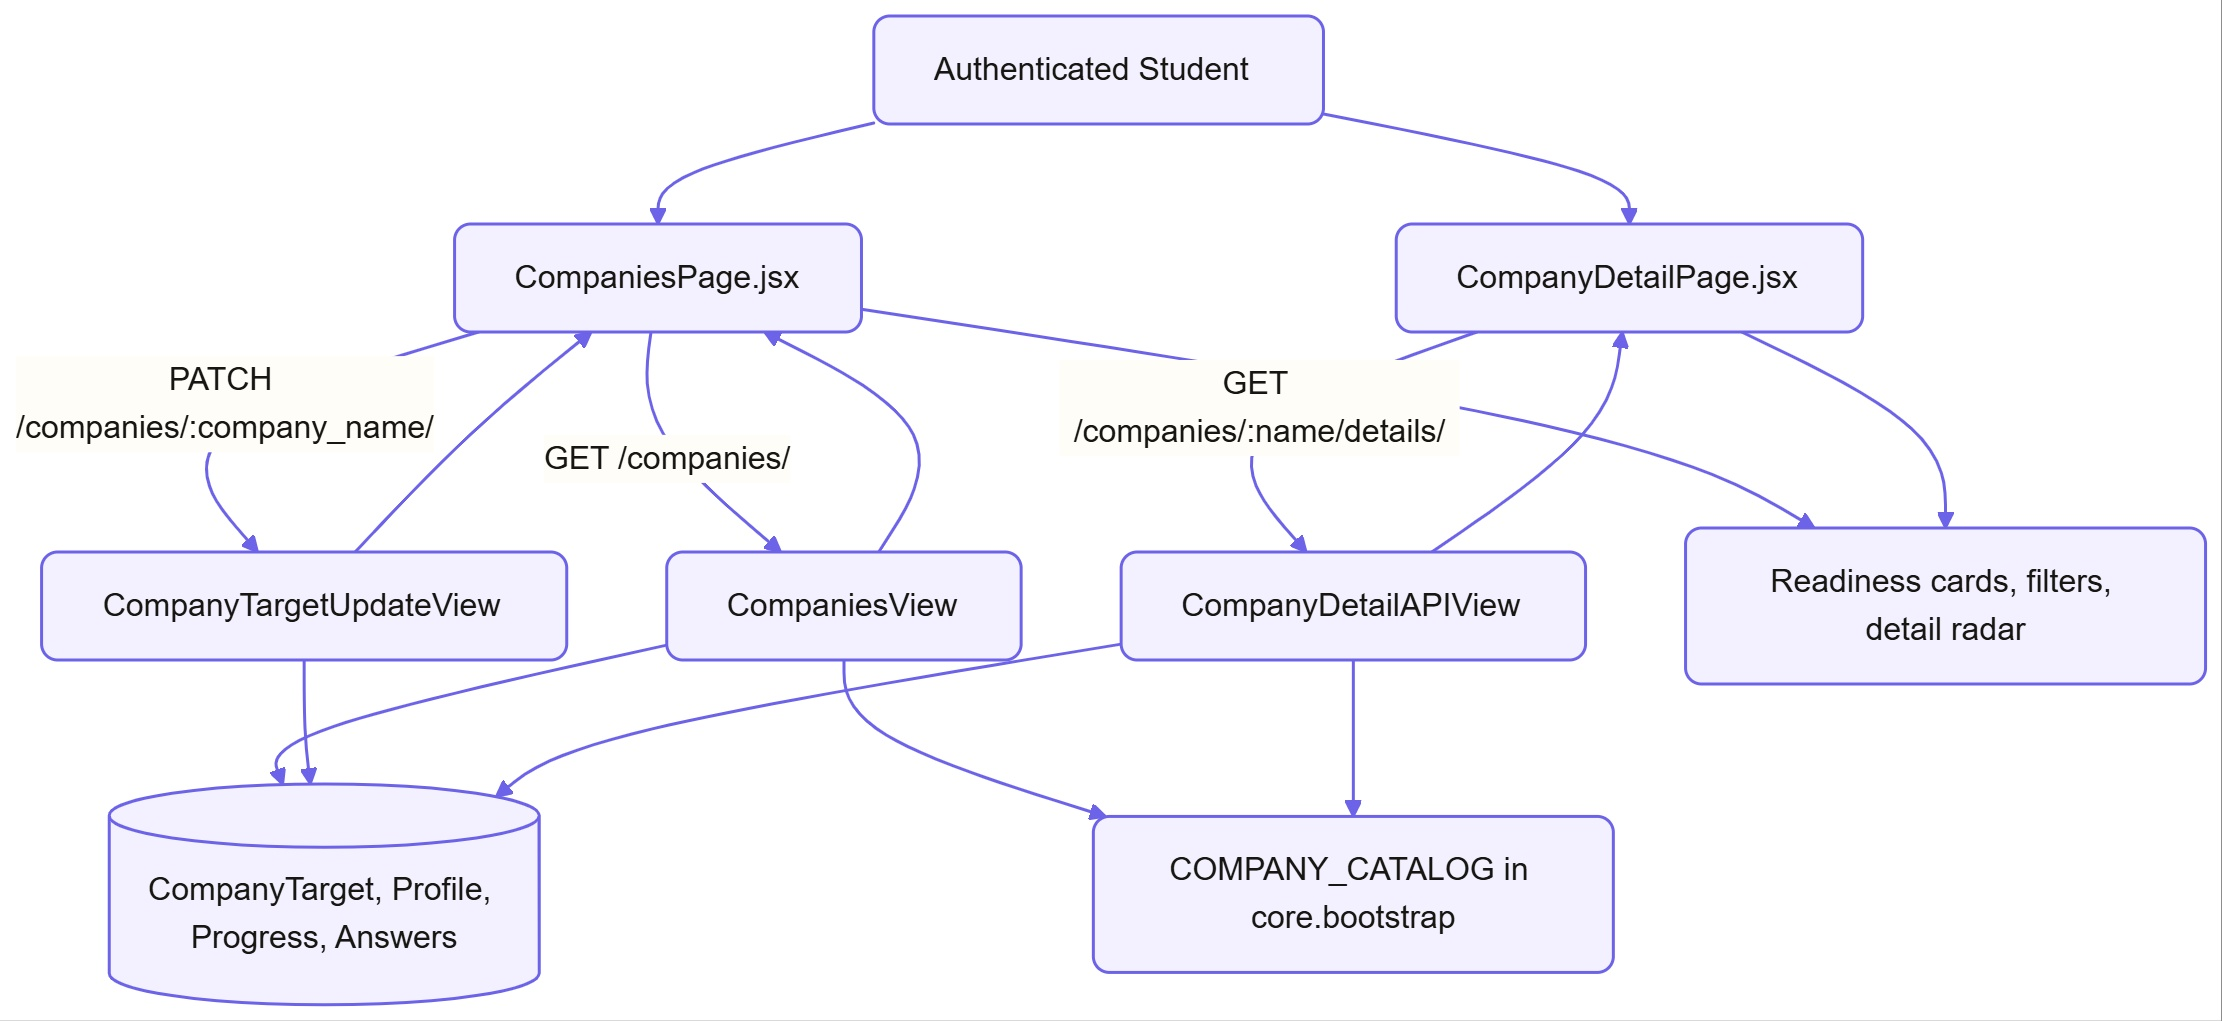
\includegraphics[width=\textwidth]{Media/Chapter 4/18 Company Readiness Workflow.jpg}
\caption{Company Readiness Workflow}
\label{fig:company_readiness_workflow}
\end{figure}

The Company Readiness Module begins when an authenticated student selects a target company through the frontend interface. The React application requests company-specific information from the backend, including preparation requirements, recommended topics, coding difficulty, interview expectations, and readiness metrics.

The backend retrieves the selected company's preparation profile together with the student's learning progress, coding submissions, quiz performance, interview results, and completed learning topics. These records are analyzed to calculate the student's readiness level for the selected company.

Based on the calculated readiness score, the module identifies completed requirements, pending topics, weak subject areas, and recommended activities. The generated information is returned to the frontend, where it is presented using progress indicators, readiness cards, and detailed preparation summaries.

Whenever the student completes additional learning activities, coding problems, or mock interviews, the readiness score is automatically recalculated, ensuring that the displayed information always reflects the student's current preparation status.

\subsection{Company Readiness Workflow}

The Company Readiness Module follows the sequence below.

\begin{enumerate}

\item The student selects a target company.

\item The frontend requests company preparation details.

\item The backend retrieves the student's preparation records.

\item Company requirements are compared with the student's progress.

\item Readiness scores are calculated.

\item Weak areas and pending topics are identified.

\item Personalized recommendations are generated.

\item The frontend displays the updated company readiness dashboard.

\end{enumerate}

\subsection{Major Features}

The Company Readiness Module provides the following features.

\begin{itemize}

\item Company-specific preparation tracking.

\item Personalized readiness score calculation.

\item Topic recommendation based on company requirements.

\item Coding readiness analysis.

\item Interview readiness evaluation.

\item Progress visualization.

\item Automatic readiness updates.

\item Integration with dashboard analytics.

\end{itemize}

\subsection{Advantages of the Company Readiness Module}

The implemented module provides several advantages.

\begin{itemize}

\item Supports focused preparation for individual companies.

\item Helps students identify preparation gaps.

\item Provides personalized learning recommendations.

\item Continuously updates readiness scores.

\item Integrates multiple preparation activities into a unified evaluation.

\item Improves placement preparation efficiency.

\end{itemize}

\section{Chapter Summary}

This chapter described the implementation of the PrepSmart platform, including the technologies, development environment, frontend architecture, backend architecture, authentication mechanism, placement preparation workflow, dashboard analytics, mock test module, AI interview module, coding practice environment, portfolio and skills passport generation, and company readiness module.

The implementation follows a modular client--server architecture developed using React, Django, Django REST Framework, and MySQL. The integration of AI-assisted interview evaluation, coding practice, personalized analytics, and company-specific preparation provides students with a comprehensive placement preparation ecosystem.

The next chapter presents the results of the developed system through screenshots of the implemented user interfaces and demonstrates the practical functionality of each module.